\documentclass[12pt]{article}
\usepackage{amsmath, amssymb, amsfonts, amsthm, mathtools,mathrsfs}
\usepackage{thmtools}
\usepackage[utf8]{inputenc}
\usepackage[inline]{enumitem}
\usepackage[colorlinks=true]{hyperref}
\usepackage{multicol}
\usepackage{witharrows}
\usepackage{tikz}
\usetikzlibrary{automata,positioning}
\usetikzlibrary{decorations.markings}
\usepackage{verbatim}
\usetikzlibrary{arrows.meta}
\usepackage{witharrows}
\usepackage[useregional, showdow]{datetime2}
\usepackage{physics}
\DTMlangsetup[en-GB]{abbr}
\usepackage{xcolor}
\usepackage[normalem]{ulem}
\usetikzlibrary{chains,shapes.multipart}

\usepackage{bbm}
\usepackage[page,toc,titletoc,title]{appendix}
\usepackage{tocloft}
\setlength\parindent{0pt}
\usepackage{parskip}

\def\D{\mathrm{d}}
\def\P{\mathbb{P}}
\def\E{\mathbb{E}}
\def\Var{\text{Var}}
\def\F{\mathcal{F}} 
\def\ccdf{\overline{F}} 
\newcommand*{\thead}[1]{\multicolumn{1}{c}{\bfseries #1}}
\renewcommand{\arraystretch}{1}
\newcommand{\indep}{\perp \!\!\! \perp}

\usepackage[framemethod=tikz]{mdframed}
\mdfdefinestyle{theoremstyle}{%
	% linecolor=gray,linewidth=1pt,%
	% frametitlerule=true,%
	frametitlebackgroundcolor=white,
	% backgroundcolor=  gray!20,	
	bottomline=false, topline=false, rightline=false, leftline=true,
	innerlinewidth=0.7pt, outerlinewidth=0.2pt, middlelinewidth=2pt, middlelinecolor=white, %
	innerleftmargin=6pt,
	% innertopmargin=-1pt,
	skipabove=10pt,
	% fontcolor=blue,
	% innerbottommargin=-0.5pt,
}
\mdtheorem[style=theoremstyle]{defn}[thm]{Definition}[section]
\mdtheorem[style=theoremstyle]{lem}[thm]{Lemma}
\mdtheorem[style=theoremstyle]{prop}[thm]{Proposition}
\mdtheorem[style=theoremstyle]{thm}{Theorem}[section]
\mdtheorem[style=theoremstyle]{cor}{Corollary}[section]


\newcommand*{\doublerule}{\hrule width \hsize height 1pt \kern 0.5mm \hrule width \hsize height 2pt}
\newcommand{\doublerulefill}{\leavevmode\leaders\vbox{\hrule width .1pt\kern1pt\hrule}\hfill\kern0pt}
\def\ddfrac#1#2{\displaystyle\frac{\displaystyle #1}{\displaystyle #2}}


%\newcommand{\Res}{\operatorname{Res}}

\theoremstyle{definition}
% \numberwithin{thm}{section}
% \newtheorem{lem}[thm]{Lemma}
% \newtheorem{defn}[thm]{Definition}
% \newtheorem{prop}[thm]{Proposition}
% \newtheorem{cor}[thm]{Corollary}
% \newtheorem{ex}{Example}


\let\emptyset\varnothing

\usepackage{titlesec}
\titleformat{\section}[block]{\Large\filcenter\bfseries}{\S\thesection.}{0.25cm}{\Large}
\titleformat{\subsection}[block]{\large\bfseries\sffamily}{\S\S\thesubsection.}{0.2cm}{\large}

\usepackage[a4paper]{geometry}
\usepackage{lipsum}
\usepackage{xcolor,cancel}

\usepackage{cleveref}
\crefname{thm}{Theorem}{Theorems}
\crefname{lem}{Lemma}{Lemmas}
\crefname{defn}{Definition}{Definitions}
\crefname{prop}{Proposition}{Propositions}
\crefname{cor}{Corollary}{Corollaries}
\crefname{equation}{}{}
\DeclareMathOperator*{\argmin}{arg\,min}

\usepackage{mdframed}
\newenvironment{blockquote}
{\begin{mdframed}[skipabove=0pt, skipbelow=0pt, innertopmargin=4pt, innerbottommargin=4pt, bottomline=false,topline=false,rightline=false, linewidth=2pt]}
{\end{mdframed}}
\newenvironment{soln}{\begin{proof}[Solution]}{\end{proof}}

\title{Markov Chains and Queueing Systems\\}
\author{Ishan Kapnadak}
\date{Spring Semester 2020-21\\~\\Updated on: \textcolor{blue}{\DTMToday}}

\begin{document}
\tikzset{lab dis/.store in=\LabDis,
  lab dis=-0.4,
  ->-/.style args={at #1 with label #2}{decoration={
    markings,
    mark=at position #1 with {\arrow{>}; \node at (0,\LabDis) {#2};}},postaction={decorate}},
  -<-/.style args={at #1 with label #2}{decoration={
    markings,
    mark=at position #1 with {\arrow{<}; \node at (0,\LabDis)
    {#2};}},postaction={decorate}},
  -*-/.style args={at #1 with label #2}{decoration={
    markings,
    mark=at position #1 with {{\fill (0,0) circle (1.5pt);} \node at (0,\LabDis)
    {#2};}},postaction={decorate}},
  }
\maketitle

\begin{abstract}
    \begin{center}
        Lecture Notes for the course EE 621 : Markov Chains and Queueing Systems taught in Spring 2021 by Prof. Jayakrishnan Nair. Additional References include Performance Modeling and Design of Computer Systems: Queueing Theory in Action, by Mor Harchol-Balter, and Data Networks, by Dimitri Bertsekas and Robert Gallager.
    \end{center}
\end{abstract}

\tableofcontents
\newpage
\section{Introduction}

\begin{defn}[Stochastic Process]
    A \emph{stochastic process} $\left\{ X(t), t \in \mathcal{T} \right\}$ is a family of random variables indexed by a set $\mathcal{T}$.
\end{defn}

For a discrete-time stochastic process, $\mathcal{T}$ could be $\mathbb{N}$ or $\mathbb{Z}$. For a continuous-time stochastic process, $\mathcal{T}$ could be $\mathbb{R}$ or $\mathbb{R}_+$. 

\medskip

A Bernoulli random variable $X$ takes values in $\left\{ 0,1 \right\}$ with $\P\left( X = 1 \right) = p$, for some $p \in (0,1)$. Using a Bernoulli random variable, we can also define a Bernoulli \emph{process}, as follows:

\begin{defn}[Bernoulli Process]
    A \emph{Bernoulli process} $\left\{ X_n, n \in \mathbb{N} \right\}$ is a sequence of \emph{i.i.d} (independent and identically distributed) Bernoulli random variables with parameter $p$. We denote a Bernoulli process with parameter $p$ as $BP(p)$.
\end{defn}

The sample path of a Bernoulli process is essentially a binary sequence. An example of a sample path could be
\[
    1, \, 0, \, 1, \, 1, \, 0, \, 0, \cdots
\]

A $1$ in a sample path can be thought of as a `success' or an `arrival' or something else based on context. Since this is a course on queueing theory, we shall call the $1$'s as \emph{arrivals}. For a given Bernoulli process, we define a few important parameters associated with it. 

\begin{enumerate}
    \item We define $A_1$ to be the time of the first arrival. That is,
    \[
        A_1 = \min \left\{ n \geq 1 \colon X_n = 1 \right\}
    \]
    An interesting question to ask now would be that what is the distribution of $A_1$. It turns out that $A_1$ is a \emph{geometric random variable}. Specifically, we have
    \[
        \P\left( A_1 = k \right) = \left( 1 - p \right)^{k-1} \cdot p \quad \text{and} \quad \mathbb{E}[A_1] = \frac{1}{p}
    \]
    We shall write $A_1 \sim \text{Geometric}(p)$.
    
    \item We also define $N(t)$ to be the number of arrivals until time $t$. It is easy to see that the $N(t)$ has a \emph{binomial} distribution with parameters $t$ and $p$. Specifically, we have
    \[
        \P \left( N(t) = k \right) = \binom{t}{k} \cdot p^k \cdot \left( 1-p \right)^{t-k}
    \]
    We shall write $N(t) \sim \text{Binomial}(t, p)$.
    
    \item We denote $A_k$ as the time of the $k^{\text{th}}$ arrival. For $k \geq 2$, we then define
    \[
        T_k = A_k - A_{k-1}
    \]
    which are the \emph{inter-arrival times} of the Bernoulli process. It is also easy to show that $T_k \sim \text{Geometric}(p)$. This allows us to define a Bernoulli process alternatively as

\begin{defn}[Bernoulli Process]
    A Bernoulli process with parameter $p$ is a $\{0,1\}$ random process with \emph{i.i.d} Geometric$(p)$ inter-arrival times.
\end{defn}
\end{enumerate}

We shall now state a few important properties of Bernoulli processes. 

\begin{enumerate}
    \item \underline{Splitting:} Consider a $BP(p)$. Each arrival of the process is made part of Stream A with probability $q$ and part of Stream B with probability $1-q$. That is, the Bernoulli process is `split' into two streams with a fixed probability parameter $q$. Now, Stream A and Stream B are arrival processes in their own rights. It turns out that these two split streams are Bernoulli processes as well. Further, Stream A is $BP(pq)$ and Stream B is $BP(p(1-q))$. However, these two streams are not independent processes. In particular, they both cannot have an arrival at the same time!
    
    \item \underline{Merging:} Consider a $BP(p)$ and a $BP(q)$ which are mutually independent. We merge the two processes as follows: An arrival occurs in the merged process if one occurs in either or both of the original processes. Then, the merged process is also a Bernoulli process and it has parameter $p+q-pq$.
    
    \item Finally, we have that the Bernoulli process is \emph{independent} and \emph{stationary}. It is thus, one of the simplest stochastic processes. 
\end{enumerate}

\newpage\section{Discrete Time Markov Chains}

\subsection{What is a DTMC?}

We shall now move on to define a DTMC. First, we will recall two important notions from probability, namely - independence and conditional independence. 

\begin{defn}[Independence]
    Two events $A$ and $B$ are said to be \emph{independent} if 
    \[
        \P \left( A \mid B \right) = \P \left( A \right) \textcolor{blue}{\iff \P \left( B \mid A \right) = \P \left( B \right)}
    \]
\end{defn}
Note: Here, we have implicitly assumed that all these conditional probabilities are indeed defined. That is, we have assumed that $\P(A)$ and $\P(B)$ are positive.

\begin{defn}[Conditional Independence]
    Two events $A$ and $B$ are said to be independent \emph{conditioned on $C$} (or given $C$), if 
    \[
        \P \left( A \mid BC \right) = \P \left( A \mid C \right) \textcolor{blue}{\iff \P \left( B \mid AC \right) = \P \left( B \mid C \right)}
    \]
    where $AC$ denotes $A \cap C$ and $BC$ denotes $B \cap C$.
\end{defn}
Here again, we have assumed that all conditional probabilities are well defined. That is, we have assumed that $\P(C)$, $\P(AC)$ and  $\P(BC)$ are positive. We can now define a DTMC. 

\begin{defn}[Discrete Time Markov Chain (DTMC)]
    Let $S$ denote a countable set. A random process $\left\{ X_n \right\}_{n \geq 0}$ taking values in $S$ is said to be a \emph{Discrete Time Markov Chain (DTMC)} if for all $n$ and for all $i_0, i_1, i_2, \ldots , i, j \in S$, we have
    \[
        \P \left( X_{n+1} = j \mid X_0 = i_0, X_1 = i_1, X_2 = i_2, \ldots ,X_n = i \right) = \P \left( X_{n+1} = j \mid X_n = i \right)
    \]
\end{defn}

The set $S$ is called the state space of the DTMC. Further, we will denote the above probability (the probability of transitioning from state $i$ to state $j$ at time $n$) as $p_{ij}(n)$ and we will refer to these as \emph{transition probabilities}.

\medskip

Intuitively, for a DTMC, the next state of the process is independent of the past states of the process when conditioned on the present state. In other words, the next state of the process only depends on its current state and not on the history (or past states) of the process. 

\medskip

As an example, suppose $\left\{ Y_n \right\}_{n \geq 1}$ is a $BP(p)$. We define $X_0 = 0$ and 
\[
    X_n = X_{n-1} + Y_n
\]
for $n \geq 1$. Then, $\left\{X_n\right\}$ defines a \emph{random walk} on $\mathbb{Z}_+$. At each time instant, the process ``moves right'' with probability $p$ and ``stays put'' with probability $(1-p)$. We now claim that $\{ X_n \}$ is a DTMC over $\mathbb{Z}_+$. Indeed, we have
\[
    \P \left( X_{n+1} = j \mid X_0 = i_0, X_1 = i_1, X_2 = i_2, \ldots ,X_n = i \right)
\]
\[
    = \begin{cases}
        p & j = i+1 \\
        1-p & j = i \\
        0 & \text{otherwise}
    \end{cases}
\]
These transition probabilities are clearly dependent only on the present state $i$, validating our claim.

\medskip

For most applications, we would be dealing with \emph{time-homogeneous} DTMCs - that is, DTMCs for which the transition probabilities are independent of time. For time-homogeneous DTMCs, it suffices to denote the transition probabilities as simply $p_{ij}$. We may represent time-homogeneous DTMCs pictorially via a \emph{transition probability diagram (TPD)}. The TPD for the random walk example is shown below

\begin{center}
    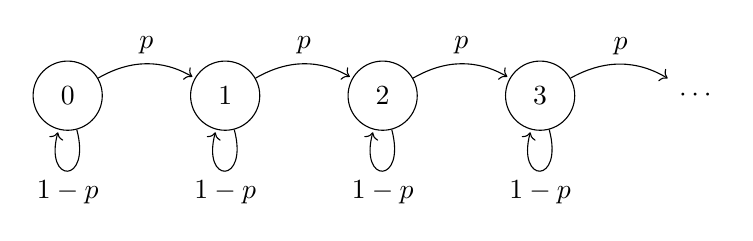
\begin{tikzpicture}[shorten >=1pt,node distance=2cm,on grid,auto] 
   \node[state] (q_0)   {$0$}; 
   \node[state] (q_1) [right=of q_0] {$1$}; 
   \node[state] (q_2) [right=of q_1] {$2$}; 
   \node[state] (q_3) [right=of q_2] {$3$};
   \node[draw=none] (q_dot) [right=of q_3] {$\cdots$};
    \path[->] 
    (q_0) edge [loop below] node {$1-p$} (q_0)
    (q_0) edge [bend left] node {$p$} (q_1)
    (q_1) edge [loop below] node {$1-p$} (q_1)
    (q_1) edge [bend left] node {$p$} (q_2)
    (q_2) edge [loop below] node {$1-p$} (q_2)
    (q_2) edge [bend left] node {$p$} (q_3)
    (q_3) edge [loop below] node {$1-p$} (q_3)
    (q_3) edge [bend left] node {$p$} (q_dot);
\end{tikzpicture}
\end{center}

Another example where a DTMC is used is the \emph{Gilbert-Elliot Model}, which models the quality of a wireless channel as a $2$-state DTMC. The TPD for this model is shown below

\begin{center}
    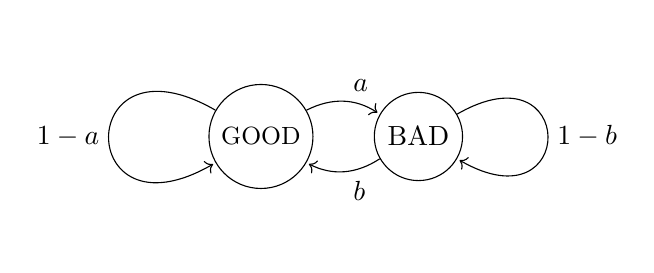
\begin{tikzpicture}[shorten >=1pt,node distance=2cm,on grid,auto] 
   \node[state] (good)   {\small{GOOD}}; 
   \node[state] (bad) [right=of good] {BAD}; 
    \path[->] 
    (good) edge[in=210, out=150] [loop] node[swap] {$1-a$} (good)
    (good) edge [bend left] node {$a$} (bad)
    (bad) edge[in=330, out=30] [loop] node {$1-b$} (bad)
    (bad) edge [bend left] node {$b$} (good);
\end{tikzpicture}
\end{center}

The TPD is a \emph{weighted directed graph} where the nodes are states and an edge from $i$ to $j$ exists if $p_{ij} > 0$. In this case, the weight of the edge is $p_{ij}$.

\medskip

We will also find it useful to ``pack'' these transition probabilities into a matrix. We define the \emph{transition probability matrix (TPM)}, $P$, as
\[
    P = \begin{bmatrix}
        p_{ij}
    \end{bmatrix}
\]
When $S$ is finite, we see that $P$ is a square matrix of size $\abs{S} \times \abs{S}$. Further, $P$ is a \emph{stochastic matrix}. That is, all the rows of $P$ sum up to $1$. This follows from the fact that
\[
    \sum_{j \in S} p_{ij} = 1 \quad \forall \, i \in S
\]

For the Gilbert-Elliot model (with `GOOD' enumerated as $1$ and `BAD' enumerated as $2$), the TPM is given by 
\[
    \begin{bmatrix}
        1-a & a \\
        b & 1-b
    \end{bmatrix}
\]
For the random walk example, $S$ is infinite. However, the matrix $P$ may be visualised as follows
\[
    \begin{bmatrix}
        1-p & p & 0 & 0 & 0 & \cdots \\
        0 & 1-p & p & 0 & 0 & \cdots \\
        0 & 0 & 1-p & p & 0 & \cdots \\
        0 & 0 & 0 & 1-p & p & \cdots \\
        \vdots & \vdots & \vdots & \vdots & \vdots & \ddots
    \end{bmatrix}
\]

That is, the TPM corresponding to the random walk example has $(1-p)$ along its diagonal and $p$ along its superdiagonal.

\subsection{The Law of a DTMC}

We now wish to find the \emph{law} or distribution of a DTMC. Given a DTMC $\left\{ X_n \right\}_{n \geq 0}$, we specify its law by specifying the joint distribution of every finite subset of random variables. It turns out that the very definition of a DTMC leads to a neat and compact way of expressing this law. First, we will understand the $n$-step transition probabilities. Recall that we had defined
\[
    p_{ij} \vcentcolon= \P \left( X_1 = j \mid X_0 = i \right) = \P \left( X_{m+1} = j \mid X_m = i \right)
\]
as the $1$-step transition probabilities and $P \vcentcolon= \begin{bmatrix}
    p_{ij}
\end{bmatrix}$ as the $1$-step TPM. Similarly, for $n \geq 1$, we define
\[
    p_{ij}^{(n)} \vcentcolon= \P \left( X_n = j \mid X_0 = i \right) = \P \left( X_{n+m} = j \mid X_m = i \right)
\]
as the $n$-step transition probabilities and $P^{(n)} \vcentcolon= \begin{bmatrix}
    p_{ij}^{(n)}
\end{bmatrix}$ as the $n$-step TPM. Notice that $p_{ij}^{(1)} = p_{ij}$ for all $i,j$ and $P^{(1)} = P$. We will now try to explicitly calculate these probabilities for the case $n=2$. We have

\[
    \begin{WithArrows}[displaystyle]
		p_{ij}^{(2)} &= \P \left( X_2 = j \mid X_0 = i \right) \Arrow{Total Probability Law} \\
		&= \sum_{k} \P \left( X_2 = j, X_1 = k \mid X_0 = i \right) \\
		&= \sum_{k} \P \left( X_1 = k \mid X_0 = i \right) \cdot \P \left( X_2 = j \mid X_1 = k, X_0 = i \right) \Arrow{Markov Property} \\
		&= \sum_{k} \P \left( X_1 = k \mid X_0 = i \right) \cdot \P \left( X_2 = j \mid X_1 = k \right)
	\end{WithArrows}
\]
\[
    \therefore \, p_{ij}^{(2)} = \sum_{k} p_{ik} \cdot p_{kj}
\]
The above expression looks \emph{exactly} like a matrix multiplication. In fact, you should be able to convince yourself that
\[
    P^{(2)} = P \cdot P \implies P^{(2)} = P^2
\]

For $n=3$, we have
\[
    \begin{WithArrows}[displaystyle]
		p_{ij}^{(3)} &= \P \left( X_3 = j \mid X_0 = i \right) \Arrow{Total Probability Law} \\
		&= \sum_{k} \P \left( X_3 = j, X_2 = k \mid X_0 = i \right) \\
		&= \sum_{k} \P \left( X_2 = k \mid X_0 = i \right) \cdot \P \left( X_3 = j \mid X_2 = k, X_0 = i \right) \Arrow{Markov Property} \\
		&= \sum_{k} \P \left( X_2 = k \mid X_0 = i \right) \cdot \P \left( X_3 = j \mid X_2 = k \right)
	\end{WithArrows}
\]
\[
    \therefore \, p_{ij}^{(3)} = \sum_{k} p^{(2)}_{ik} \cdot p_{kj}
\]
Thus, we get
\[
    P^{(3)} = P^{(2)} \cdot P \implies P^{(3)} = P^3
\]

Inductively, one can then show that 
\[
    \boxed{P^{(n)} = P^n \quad \forall \, n \in \mathbb{N}}
\]

We now claim that the law of a DTMC $\left\{ X_n \right\}_{n \geq 0}$ can be completely specified in terms of 
\begin{enumerate}
    \item The law or distribution of $X_0$, specified as a row vector $\mu_0$ with \[\mu_0(i) = \P \left( X_0 = i \right)\]
    \item The transition probability matrix, $P$.
\end{enumerate}

Before we proceed to show this, let us first examine the law of $X_n$. That is, we wish to find $\mu_n$ in terms of $\mu_0$ and $P$. We have
\[
    \begin{WithArrows}[displaystyle]
		\mu_n(j) &= \P \left( X_n = j \right) \Arrow{Total Probability Law} \\
		&= \sum_{i \in S} \, \P \left( X_n = j, X_0 = i \right) \\
		&= \sum_{i \in S} \, \P \left( X_0 = i \right) \cdot \P \left( X_n = j \mid X_0 = i \right)
	\end{WithArrows}  
\]
\[
    \therefore \, \mu_n(j) = \sum_{i \in S} \, \mu_0(i) \cdot p_{ij}^{(n)}
\]
In terms of matrices, we have
\[
    \mu_n = \mu_0 \cdot P^{(n)} = \mu_0 \cdot P^n
\]

Let us now finally look at the law of the entire DTMC. Namely, we wish to specify the joint law of any finite set of $X_i$'s in terms of $\mu_0$ and $P$. Let $n_1 < n_2 < \ldots < n_m$ all be natural numbers. Let $i_1, i_2, \ldots, i_m \in S$. We wish to find 
\[
    \begin{WithArrows}[displaystyle]
    & \; \P \left( X_{n_1} = i_1, X_{n_2} = i_2, \ldots , X_{n_m} = i_m \right) \Arrow[xoffset = -2cm]{Total Probability Law} \\
    &= \sum_{i \in S} \P \left( X_0 = i, X_{n_1} = i_1, X_{n_2} = i_2, \ldots , X_{n_m} = i_m \right) \\
    &= \sum_{i \in S} \P \left( X_0 = i \right) \cdot \P \left( X_{n_1} = i_1 \mid X_0 = i \right) \cdot \P \left( X_{n_2} = i_2 \mid X_{n_1} = i_1 , X_0 = i \right) \cdots \Arrow{Markov Property} \\
    &= \sum_{i \in S} \P \left( X_0 = i \right) \cdot \P \left( X_{n_1} = i_1 \mid X_0 = i \right) \cdot \P \left( X_{n_2} = i_2 \mid X_{n_1} = i_1 \right) \cdots \\
    &= \sum_{i \in S} \mu_0(i) \cdot p_{ii_1}^{(n_1)} \cdot p_{i_1i_2}^{(n_2 - n_1)} \cdot \ldots \cdot p_{i_{m-1}i_m}^{(n_{m-1} - n_m)}
    \end{WithArrows}
\]

Although the notation is cumbersome, we see that we can specify the joint distribution of any finite set of $X_i$'s in terms of only $\mu_0$ and $P$.


\subsection{The long-run behaviour of a DTMC}

To study the long-run behaviour of a DTMC, we make use of three important distributions associated with a DTMC. 

\medskip

\begin{defn}[Limiting Distribution]
    Consider a DTMC over state space $S$. A probability distribution $l = \begin{bmatrix}
        l_1 & l_2 & \cdots
    \end{bmatrix}$ is called a \emph{limiting distribution} of the DTMC if
    \[
        \lim_{n \to \infty} p_{ij}^{(n)} = l_j \quad \forall \, i,j \in S
    \]  
\end{defn}

In other words, as $n$ grows larger, the $n$-step transition probabilities to a state $j$ converge to $l_j$ regardless of the initial state.

\begin{defn}[Time-average Distribution]
    Consider $\left\{ X_n \right\}_{n \geq 0}$ to be a DTMC over state space $S$. The probability distribution $\theta = \begin{bmatrix}
        \theta_1 & \theta_2 & \cdots
    \end{bmatrix}$ is called the \emph{time-average distribution} of the DTMC if
    \[
        \lim_{n \to \infty} \, \frac{1}{n} \, \sum_{i = 1}^{n} \mathbbm{1}_{\left\{X_i = j\right\}} \, = \theta_j \quad \text{almost surely}
    \]
\end{defn}

Here $\mathbbm{1}$ represents the \emph{indicator function}. Intuitively, the time-average distribution captures the average fraction of time spent by the DTMC in each state.

\begin{defn}[Stationary Distribution]
    Consider a DTMC with a transition probability matrix $P$. A probability distribution $\pi = \begin{bmatrix}
        \pi_1 & \pi_2 & \cdots
    \end{bmatrix}$ is called a \emph{stationary distribution} of the DTMC if 
    \[
        \pi = \pi \cdot P
    \]
    $\pi$ is sometimes also called an \emph{invariant distribution}
\end{defn}

If the initial law of the DTMC is $\mu_0 = \pi$, then it is trivial to see that $\mu_n = \pi$ for all $n \in \mathbb{N}$. Hence, the process remains stationary when the initial law is given by the stationary distribution. In many applications, we find that $l = \pi = \theta$. We will now try to reason about when these three distributions exist and when are they equal. 

\begin{thm} \label{thm:limstat}
    Consider a DTMC over state space $S$. If the DTMC has a limiting distribution $l$, then $l$ is also a stationary distribution. Moreover, $l$ is the only stationary distribution.
\end{thm}

To prove the following theorem, we first state and prove the following short lemma. 

\begin{lem} \label{lem:lim}
    Consider a DTMC over state space $S$ which has a limiting distribution $l$. For any initial law $\mu_0$, $\mu_n \to l$ pointwise.
\end{lem}

\begin{proof}[Proof of Lemma \ref{lem:lim}]
    We know 
    \[
        \mu_n(j) = \P \left( X_n = j \right) = \sum_{i \in S} \mu_0(i) \cdot p_{ij}^{(n)} \quad \forall \, j \in S
    \]
    First consider that $S$ is finite. It then follows that
    \begin{align*}
        \lim_{n \to \infty} \mu_n(j) &= \lim_{n \to \infty} \sum_{i \in S} \mu_0(i) \cdot p_{ij}^{(n)} = \sum_{i \in S} \mu_0(i) \cdot \left( \lim_{n \to \infty} p_{ij}^{(n)} \right) \\
        &= \sum_{i \in S} \mu_0(i) \cdot l_j = l_j \cdot \sum_{i \in S} \mu_0(i) = l_j \cdot 1
    \end{align*}
    \[
        \therefore \, \lim_{n \to \infty} \mu_n(j) = l_j
    \]
    as desired. The proof for an infinite state space is slightly trickier since we cannot interchange sum and limits without justification. Consider now that $S$ is infinite. We now have
    \[
        \mu_n(j) = \sum_{i = 1}^{\infty} \mu_0(i) \cdot p_{ij}^{(n)}
    \]
    Also, it is easy to see that
    \[
        \sum_{i=1}^{M} \mu_0(i) \cdot p_{ij}^{(n)} \, \leq \, \mu_n(j) \, \leq \, \sum_{i=1}^{M} \mu_0(i) \cdot p_{ij}^{(n)} + \sum_{i=M+1}^{\infty} \mu_0(i)
    \]
    for any $M \in \mathbb{N}$. Letting $n$ go to $\infty$, we see that
    \[
        l_j \cdot \sum_{i = 1}^{M} \mu_0(i) \, \leq \, \liminf_{n \to \infty} \, \mu_n(j) \, \leq \, \limsup_{n \to \infty} \, \mu_n(j) \, \leq \, l_j \cdot \sum_{i=1}^M \mu_0(i) + \sum_{i=M+1}^{\infty} \mu_0(i)
    \]
    Now, letting $M$ go to $\infty$, we see 
    \[
        l_j \, \leq \, \liminf_{n \to \infty} \, \mu_n(j) \, \leq \, \limsup_{n \to \infty} \, \mu_n(j) \, \leq \, l_j
    \]
    It then follows that
    \[
        \liminf_{n \to \infty} \, \mu_n(j) = \limsup_{n \to \infty} \, \mu_n(j) = l_j
    \]
    and thus
    \[
        \lim_{n \to \infty} \mu_n(j) = l_j
    \]
    as desired.
    
    
\end{proof}

We now begin our proof of Theorem \ref{thm:limstat}. Note that we will have to prove the theorem in two parts - first, we will show that if a limiting distribution exists, then it is stationary. Second, we will show that this limiting distribution is in fact the unique stationary distribution.

\begin{proof}[Proof of Theorem \ref{thm:limstat}]
    We will first show that $l = l \cdot P$ where $l$ is the limiting distribution of the DTMC. We have
    \[
        p_{ij}^{(n)} = \sum_{k \in S} p_{ik}^{(n-1)} \cdot p_{kj}
    \]
    
    If $S$ is finite, then taking limits on either side, we get
    \[
        \lim_{n \to \infty} p_{ij}^{(n)} = \sum_{k \in S} \, \left[ \lim_{n \to \infty} \, p_{ik}^{(n-1)} \right] \cdot p_{kj}
    \] 
    \[
        \therefore \, l_j = \sum_{k \in S} l_k \cdot p_{kj} \implies l = l \cdot P
    \]
    Once again, this proof does not work when $S$ is infinite. If $S$ is infinite, we note that
    \[
        p_{ij}^{(n)} = \sum_{k=1}^{\infty} p_{ik}^{(n-1)} \cdot p_{kj}
    \]
    For any $M \in \mathbb{N}$, we see that
    \[
        p_{ij}^{(n)} \geq \, \sum_{k=1}^{M} p_{ik}^{(n-1)} \cdot p_{kj}
    \]
    Now, letting $n \to \infty$, we see
    \[
        l_j \geq \, \sum_{k=1}^{M} l_{k} \cdot p_{kj}
    \]
    for all $M \in \mathbb{N}$. Next, letting $M \to \infty$, we see that
    \[
        l_j \geq \, \underbrace{\sum_{k=1}^{\infty} l_k \cdot p_{kj}}_{\alpha_j} \quad \forall \, j \in S
    \]  
    Note that 
    \[
        \sum_{j =1}^{\infty} l_j = 1
    \]  
    and
    \[
        \sum_{j=1}^{\infty} \alpha_j = \sum_{j=1}^{\infty} \sum_{k=1}^{\infty} l_k \cdot p_{kj} = \sum_{k=1}^{\infty} l_k \sum_{j=1}^{\infty} p_{kj} = 1
    \]
    We know that $l_j \geq \alpha_j$ for all $j \in S$ and yet
    \[
        \sum_{j=1}^{\infty} l_j = \sum_{j=1}^{\infty} \alpha_j 
    \]
    Thus, we get that $l_j = \alpha_j$ for all $j \in S$. Thus, 
    \[
        l_j = \sum_{k=1}^{\infty} l_k \cdot p_{kj} \implies l = l \cdot P
    \]
    as desired. Next, we show that $l$ is the only stationary distribution. Let $\pi$ be any stationary distribution of the DTMC. Consider $\mu_0 = \pi$. It then follows that $\mu_n = \pi$ for all $n \in \mathbb{N}$. Letting $n \to \infty$, we see that
    \[
        \lim_{n \to \infty} \mu_n = \pi
    \]
    However, Lemma \ref{lem:lim} tells us that
    \[
        \lim_{n \to \infty} \mu_n = l
    \]
    It then follows that $\pi = l$ and hence, $l$ is the unique stationary distribution.
\end{proof}

\newpage

We now talk about two conditions which seem to be necessary for a DTMC to \emph{have} a limiting distribution. The first of these conditions is called \emph{irreducibility} which, in simple words, states that every state in the DTMC must be reachable from every other state. Why is this important? Consider the following DTMC :

\begin{center}
    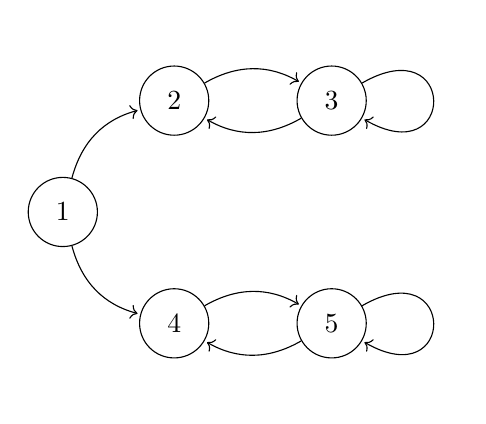
\begin{tikzpicture}[shorten >=1pt,node distance=2cm,on grid,auto] 
   \node[state] (q1)   {1}; 
   \node[state] (q2) [above right=of q1] {2}; 
   \node[state] (q3) [right=of q2] {3};
   \node[state] (q4) [below right=of q1] {4};
   \node[state] (q5) [right=of q4] {5};
    \path[->] 
    (q1) edge [bend left] node {} (q2)
    (q2) edge [bend left] node {} (q3)
    (q3) edge [bend left] node {} (q2)
    (q1) edge [bend right] node {} (q4)
    (q4) edge [bend left] node {} (q5)
    (q5) edge [bend left] node {} (q4)
    (q3) edge[in=330, out=30] [loop] node {} (q3)
    (q5) edge[in=330, out=30] [loop] node {} (q5);
\end{tikzpicture}
\end{center}

If we start in state $4$, then any limiting distribution for the above DTMC can have non-zero components only for states $4$ and $5$. Similarly, if we start in state $2$, then any limiting distribution for the above DTMC can have non-zero components only for states $2$ and $3$. Since both these conditions cannot hold together, it follows that the above DTMC has no limiting distribution. The source of this problem is the fact that the states $4$ and $5$ are not reachable from the states $2$ and $3$ and vice-versa. This problem is fixed by irreducibility. We now make this more precise.

\begin{defn}[Reachability]
    In a DTMC, state $j$ is said to be \emph{reachable} from state $i$ if there exists an $n \in \mathbb{N}$ such that $p_{ij}^{(n)} > 0$.
\end{defn}
In graph-theoretic terms, the state $j$ is said to be reachable from state $i$ if there exists a directed path from node $i$ to node $j$ in the TPD of the DTMC.

\begin{defn}[Irreducibility]
    A DTMC is said to be \emph{irreducible} if all states are reachable from one another. That is, for all $(i,j) \in S \times S$, there exists an $n \in \mathbb{N}$ such that $p_{ij}^{(n)} > 0$.
\end{defn}

In graph-theoretic terms, a DTMC is said to be irreducible if its TPD is \emph{strongly connected}. Recall that we call a directed graph $G = (\mathcal{V}, \mathcal{E})$ strongly connected if there is a path in $G$ between every pair of vertices in $\mathcal{V}$. Note that it is possible that a DTMC is not irreducible yet has a limiting distribution. However, we shall see that these DTMCs can be handled with a good understanding of irreducible DTMCs. Hence, we impose irreducibility as a necessary condition.

\medskip

The second necessary condition is \emph{aperiodicity}. To illustrate this, consider the following DTMC

\begin{center}
    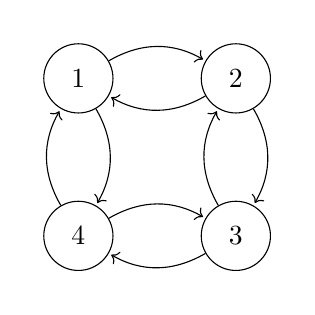
\begin{tikzpicture}[shorten >=1pt,node distance=2cm,on grid,auto] 
   \node[state] (q1)   {1}; 
   \node[state] (q2) [right=of q1] {2}; 
   \node[state] (q3) [below=of q2] {3};
   \node[state] (q4) [below=of q1] {4};
    \path[->] 
    (q1) edge [bend left] node {} (q2)
    (q2) edge [bend left] node {} (q1)
    (q3) edge [bend left] node {} (q2)
    (q2) edge [bend left] node {} (q3)
    (q4) edge [bend left] node {} (q3)
    (q3) edge [bend left] node {} (q4)
    (q4) edge [bend left] node {} (q1)
    (q1) edge [bend left] node {} (q4)
    ;
\end{tikzpicture}
\end{center}

The following DTMC cannot have a limiting distribution. Notice that $p_{12}^{(n)} = 0$ for all even $n$ and $p_{42}^{(n)} = 0$ for all odd $n$. For a limiting distribution, we must have that the limits of the above two quantities must be equal, however this can only give us a zero limit, for all states! Hence, no limiting distribution exists. This problem arises because any path from a state to itself is of even length. To deal with this problem, we introduce the idea of aperiodicity. We first define the period of a state in a DTMC. 

\begin{defn}[Period (of a state)]
    The \emph{period} of a state $j$ of a DTMC, denoted $d_j$, is defined as
    \[
        d_j \vcentcolon= \gcd{\left\{ n \colon p_{jj}^{(n)} > 0 \right\}}
    \]
    That is, the period $d_j$ of state $j$ is the GCD of all possible return path lengths to state $j$.
\end{defn}

In the above example, all states have period $2$. We also have the following interesting lemma. 

\begin{lem} \label{lem:irrstate}
    In an irreducible DTMC, all states have the same period, which is referred to as the period of the DTMC. 
\end{lem}

We then define an aperiodic DTMC as follows

\begin{defn}[Aperiodicity]
    An irreducible DTMC is called \emph{aperiodic} if it has a period $1$.
\end{defn}

Notice that an irreducible DTMC is aperiodic if \emph{any} state $i$ has a self loop ($p_{ii} > 0$).

\begin{proof}[Proof of Lemma \ref{lem:irrstate}]
    Consider two distinct states $i,j$. We wish to prove that $d_i = d_j$. By irreducibility, there exist $r, s \in \mathbb{N}$ such that $p_{ij}^{(r)} > 0$ and $p_{ji}^{(s)} > 0$. Notice now that $p_{ii}^{(r+s)} > 0$ and $p_{jj}^{(r+s)} > 0$. Let $m \mid n$ denote that $m$ divides $n$. Next, we define
    \[
        N_i \vcentcolon= \left\{ n \colon p_{ii}^{(n)} > 0 \right\}
    \]
    \[
        N_j \vcentcolon= \left\{ n \colon p_{jj}^{(n)} > 0 \right\}
    \]
    We then have that $d_i = \gcd(N_i)$ and $d_j = \gcd(N_j)$. Now, we define
    \[
        N_j^{\prime} \vcentcolon= \left\{ r+s+n \colon p_{ii}^{(n)} > 0 \right\}
    \]
    Observe that $N_j^{\prime} \subseteq N_j$. Hence, $d_j$ divides every element of $N_j^{\prime}$. That is,
    \[
        d_j \mid r+s+n \quad \forall \, n \in N_i
    \]
    But since $r+s \in N_j$, we see that $d_j \mid r+s$. Hence, 
    \[
        d_j \mid n \quad \forall \, n \in N_i
    \]
    Thus, it follows that $d_i \geq d_j$. Using similar arguments, we also see that $d_i \leq d_j$. This implies that $d_i = d_j$, as desired.
\end{proof}

We now state our first concrete result about when a limiting distribution exists. 

\begin{thm} \label{thm:finite}
    A finite, irreducible, aperiodic DTMC has a limiting distribution with strictly positive entries
\end{thm}

We state two lemmas (Lemma \ref{lem:number} and Lemma \ref{num_dtmc}) before proceeding to prove Theorem \ref{thm:finite}. 

\begin{lem} \label{lem:number}
    Let $A \subseteq \mathbb{N}$ such that 
    \begin{enumerate}
        \item $\gcd(A) = 1$
        \item $A$ is closed under addition. That is, $m, n \in A \implies m+n \in A$.
    \end{enumerate}
    
    Then, $\exists \, n_0 \in \mathbb{N}$ such that $n \in A$ for all $n \geq n_0$.
\end{lem}

A proof of this Lemma is given below and may be skipped. 

\begin{proof}[Proof of Lemma \ref{lem:number}]
    We begin the proof by first stating and proving two more lemmas. 
    
    \begin{lem} \label{lem:1.1_num}
        Let $S \subset \mathbb{Z}$ contain at least one non-zero element and be closed under addition and subtraction. Then $S$ contains a least positive element $a$ and $S = \left\{ ka \colon k \in \mathbb{Z} \right\}$
    \end{lem}
    
    \begin{proof}[Proof of Lemma \ref{lem:1.1_num}]
        Let $c \in S$, $c \neq 0$. Then, $c-c = 0 \in S$ and $0-c = -c \in S$. By trichotomy, $S$ contains at least one positive element. Let $a$ denote the smallest positive element of $S$. Since $S$ is closed under addition and subtraction, we see that $\left\{ ka \colon k \in \mathbb{Z} \right\} \subseteq S$. Let $c \in S$. Then, $c = ka + r$ where $k \in \mathbb{Z}$ and $0 \leq r < a$. Since $r = c - ka \in S$, we cannot have $r > 0$ since this would contradict $a$ being the smallest positive element. Hence, we have $r=0$ which gives $c=ka$. Thus, $S \subseteq \left\{ ka \colon k \in \mathbb{Z} \right\}$. This completes the proof.
    \end{proof}
    
    \begin{lem} \label{lem:1.2_num}
        Let $a_1, \ldots, a_k$ be positive integers with gcd $d$. Then, there exist $n_1, \ldots, n_k \in \mathbb{Z}$ such that $d = \sum_{i=1}^{k} n_i a_i$.
    \end{lem}
    
    \begin{proof}[Proof of Lemma \ref{lem:1.2_num}]
        The set $S = \left\{ \sum_{i=1}^k n_i a_i \colon n_1, \ldots, n_k \in \mathbb{Z} \right\}$ is closed under addition and subtraction. Thus, by Lemma \ref{lem:1.1_num}, $S = \left\{ ka \colon k \in \mathbb{Z} \right\}$ where $a = \sum_{i=1}^k n_i a_i$ is the smallest positive integer in $S$. Since $d$ divides all $a_i$'s, $d$ divides $a$ and hence $0 < d \leq a$. Also, each $a_i \in S$ and is therefore a multiple of $a$. Hence, $a \leq \gcd\left( a_1, \ldots, a_k \right) = d$. Therefore, $d = a$. 
    \end{proof}
    
    We now proceed to prove Lemma \ref{lem:number}. For some $k$, $1 = \gcd\left( a_1, \ldots, a_k \right)$ where $a_1, \ldots, a_k \in A$. Thus, by Lemma \ref{lem:1.2_num}, 
    \[
        1 = \sum_{i=1}^k n_i a_i
    \]
    for some $n_1, \ldots, n_k \in \mathbb{Z}$. Separating the positive and negative terms in the above equality, we have $1 = M - P$ where $M, P \in A$. Let $n \in \mathbb{N}$ such that $n \geq P(P-1)$. We have $n = aP + r$ where $r \in [0, P-1]$. We necessarily have $a \geq P-1$, otherwise if $a \leq P-2$ then we have $n = aP+r < P(P-1)$. Using $1 = M-P$, we have $n = aP + r(M-P) = (a-r)P + rM$. But $a-r \geq 0$ and hence $n \in A$. Thus, we have shown that any $n$ sufficiently large (larger than $P(P-1)$ to be precise) lies in $A$, as desired.
\end{proof}

Lemma \ref{lem:number} when applied to DTMCs, gives us the following lemma. 

\begin{lem} \label{num_dtmc}
    Given a finite, irreducible, aperiodic DTMC, $\exists \, n_0 \in \mathbb{N}$ such that $P^n > 0$ for all $n \geq n_0$. That is, every entry of $P^n$ is strictly positive for all $n \geq n_0$.
\end{lem}

\begin{proof}[Proof of Lemma \ref{num_dtmc}]
    Pick an $i \in S$. Define
    \[
        N_i \vcentcolon= \left\{ n \colon p_{ii}^{(n)} > 0 \right\}
    \]
    By aperiodicity, $\gcd(N_i) = 1$ and by construction, $N_i$ is closed under addition. We may then use Lemma \ref{lem:number} to conclude that $\exists \, n_0(i,i) \in \mathbb{N}$ such that
    \[  
        p_{ii}^{(n)} > 0 \quad \forall \, n \geq n_0(i,i)
    \]
    Now, pick another state $j \neq i$. By irreducibility, $\exists \, r \in \mathbb{N}$ such that $p_{ij}^{(r)} > 0$. It is then easy to observe that
    \[
        p_{ij}^{(n)} > 0 \quad \forall \, n \geq \underbrace{n_0(i,i) + r}_{n_0(i,j)}
    \]
    Next, we define
    \[
        n_0 \vcentcolon= \max_{i,j} \, n_0(i,j)
    \]
    Then, we see that
    \[
        p_{ij}^{(n)} > 0 \quad \forall \, i, j \in S, \quad \forall \, n \geq n_0
    \]
    Thus, $P^n > 0$ for all $n \geq n_0$.
\end{proof}

\begin{proof}[Proof of Theorem \ref{thm:finite}]
    Pick any $j \in S$. We will track the $j^{\text{th}}$ column of $P^n$, and show that it converges to a constant column. Let $e_n$ denote the $j^{\text{th}}$ column of $P^n$. We know that $P^{n+1} = P \cdot P^n$. It then follows that
    \[
        e_{n+1} = P \cdot e_n
    \]
    
    Let $M_n$ denote the maximum entry of $e_n$ and let $m_n$ denote the minimum entry of $e_n$. Since $P$ is a stochastic matrix, the entries of $e_{n+1}$ are weighted averages of entries of $e_n$. Thus, it follows that
    \[
        M_{n+1} \leq M_n \quad \text{and} \quad m_{n+1} \geq m_n \quad \forall \, n \in \mathbb{N}
    \]
    That is, $(M_n)$ is a decreasing sequence and $(m_n)$ is an increasing sequence. It is also trivial that both these sequences are bounded. Thus, $(M_n)$ and $(m_n)$ converge. Now, we define
    \[
        \Delta_n \vcentcolon= M_n - m_n
    \]
    Observe that $(\Delta_n)$ is also convergent. By Lemma \ref{num_dtmc}, $\exists \, n_0 \in \mathbb{N}$ such that $P^{n_0} > 0$. Let $S$ denote the minimum entry of $P^{n_0}$. We know that
    \[
        e_{n+n_0} = P^{n_0} \cdot e_n
    \]
    That is, entries of $e_{n+n_0}$ are weighted averages of entries of $e_n$ with weights drawn from $P^{n_0}$. Notice then that the minimum possible weight we can assign to any entry of $e_n$ is $S$. Thus, the maximum possible entry of $e_{n+n_0}$ will be no more than the value obtained by assigning a weight of $S$ to $m_n$ and a weight of $(1-S)$ to $M_n$. Similarly, the minimum entry of $e_{n+n_0}$ will be no less than the value obtained by assigning a weight of $(1-S)$ to $m_n$ and $S$ to $M_n$. That is, the following two inequalities hold
    \[
        M_{n+n_0} \leq (1-S) \cdot M_n + S \cdot m_n
    \]
    \[
        m_{n+n_0} \geq S \cdot M_n + (1-S) \cdot m_n
    \]
    Subtracting the two, we get
    \[
        \Delta_{n+n_0} \leq (1-2S) \cdot \Delta_n
    \]
    Note that $(1-2S) \in (0,1)$ (Why?). It then follows that $\Delta_n \to 0$ and hence,
    \[
        \lim_{n \to \infty} M_n = \lim_{n \to \infty} m_n =\vcentcolon l_j
    \]
    Hence, we have
    \[
        \lim_{n \to \infty} e_n \, = \begin{bmatrix}
            l_j \\ \vdots \\ l_j
        \end{bmatrix}
    \]
    which is a constant column vector, as desired. We have thus shown that the limit of $P^n$ exists and it has our desired structure (all rows are identical). It remains to show that 
    \begin{enumerate}
        \item[(i)] $\sum\limits_{j} l_j = 1$
        \item[(ii)] $l_j > 0$ for all $j \in S$
    \end{enumerate}
    
    We now prove (i). We know
    \[
        \sum_{j \in S} p_{ij}^{(n)} = 1 \quad \forall \, n \in \mathbb{N}
    \]
    Taking limit, we get
    \[
        \lim_{n \to \infty} \sum_{j} p_{ij}^{(n)} = 1
    \]
    Since the DTMC is finite, the above is a finite sum and hence, the limit can be interchanged with the sum. Thus, we have
    \[
        \sum_{j} \lim_{n \to \infty} p_{ij}^{(n)} = 1 \implies \sum_j l_j = 1
    \]
    as desired. The proof of (ii) follows from Lemma \ref{lem:stat_positive} below. 

\begin{lem} \label{lem:stat_positive}
    Let $\pi$ be a stationary distribution of an irreducible DTMC. Then, $\pi > 0$.
\end{lem}

\begin{proof}[Proof of Lemma \ref{lem:stat_positive}]
    Since $\pi$ is a stationary distribution, $\pi = \pi \cdot P$. That is,
    \[
        \pi_i = \sum_k \pi_k \cdot p_{ki}
    \]
    Suppose $\pi_i = 0$ for some $i$. From the above, it follows that $\pi_k = 0$ for all $k$ such that $p_{ki} > 0$. Proceeding inductively, we see that $\pi_k = 0$ for all $k$ such that there is a path from $k$ to $i$. Since the DTMC is irreducible, the above set is the set of all states of the DTMC, giving us $\pi = 0$ which is a contradiction (since $\pi$ is a distribution). Thus, we see that $\pi_i > 0$ for all $i \in S$.
\end{proof}


Now, note that we have already shown the existence of a limiting distribution $l$. By Theorem \ref{thm:limstat}, we have that this distribution $l$ is also stationary. Lemma \ref{lem:stat_positive} then immediately tells us that $l > 0$, completing the proof of Theorem \ref{thm:finite}.
\end{proof}

By virtue of Theorem \ref{thm:finite}, we now know that any finite, aperiodic and irreducible DTMC has a limiting distribution with strictly positive entries which equals the unique stationary distribution. To obtain this distribution, we generally solve a system of linear equations corresponding to stationarity conditions, given by
\begin{align*}
    \pi &= \pi \cdot P \\
    \sum_i \pi_i &= 1
\end{align*}

This task of finding the stationary distribution is often simplified by the use of another interesting property, known as \emph{time-reversibility}. This property is highlighted by the following theorem. 

\begin{thm}[Time-Reversibility] \label{thm:reversible}
    Given an irreducible DTMC, suppose there exists a distribution $x = \left( x_i, \; i \in S \right)$ such that
    \[
        x_i \cdot p_{ij} = x_j \cdot p_{ji} \quad \forall \, i,j \in S
    \]
    Then $x$ is a stationary distribution. In this case, we say that the DTMC is \emph{time-reversible}.
\end{thm}

Notice that we do not require the DTMC to be aperiodic or even finite. The proof for Theorem \ref{thm:reversible} is quite trivial and is illustrated below.

\begin{proof}
    We need to show that $x_i \cdot p_{ij} = x_j \cdot p_{ji} \implies x = x \cdot P$. We have
    \[
        x_i \cdot p_{ij} = x_j \cdot p_{ji} \quad \forall \, i,j \in S
    \]
    Summing over $j$, we get
    \[
        \sum_j \, x_i \cdot p_{ij} = \sum_j \, x_j \cdot p_{ji} \quad \forall \, i \in S
    \]
    Hence, 
    \[
        x_i = \sum_j \, x_j \cdot p_{ji} \quad \forall \, i \in S \implies x = x \cdot P
    \]  
\end{proof}

The reason why these chains are called time-reversible is due to the following result (proof is left as an exercise)

\begin{prop}
    Consider a time-reversible DTMC with stationary distribution $\pi$. If $\mu_0 = \pi$,then the following is true for all $i_0, \ldots , i_n \in S$ and for all $n \in \mathbb{N}$
    \[
        \P \left( X_0 = i_0, \ldots , X_n = i_n \right) = \P \left( X_0 = i_n, \ldots , X_n = i_0 \right)
    \]
\end{prop}

This result intuitively means that for a time-reversible DTMC, the probability of any finite forward trajectory is same as the probability of the reverse trajectory.

\newpage

\section{Renewal Theory}

\subsection{Introduction}

We now take a slight detour from our study of Markov chains to deal with Renewal Theory and Renewal processes. We will then apply some of the ideas from renewal theory to Markov chains. Informally, a renewal process is an arrival process with i.i.d interarrival times. More formally, we define a renewal process as the following. 

\begin{defn}[Renewal Process]
    Let $\left\{ X_i \right\}_{i \geq 1}$ be a sequence of positive, independent random random variables denoting interarrival times. Assume further that $\left\{ X_i \right\}_{i \geq 2}$ are i.i.d. Define $S_n = \sum_1^n X_i$. $S_n$ denotes the time of the $n^{\text{th}}$ arrival/renewal. For $t \geq 0$, we define
    \[
        N(t) \vcentcolon= \max \left\{ n \colon S_n(t) \leq t \right\}
    \]
    The random process $N(t)$ is called a \emph{renewal process} and denotes the number of arrivals or renewals in the interval $(0,t]$. We further define $m(t) = \mathbb{E} \left[ N(t) \right]$ to denote the expected number of arrivals in the interval $(0,t]$.
\end{defn}

These arrivals or renewals may be the arrival of buses at a bus stop, the arrival of customers to a queue, failure instants of a component in a machine, instants of Facebook posts by an individual, etc. We now make a few remarks about the definition. 

\begin{itemize}
    \item $X_1$ may have a different distribution compared to $\left\{ X_i \right\}_{i \geq 2}$ because $X_1$ may not be a true interarrival time. It is simply the time of the first arrival since observation began. 
    \item Since all $X_i$'s are positive, we don't have multiple arrivals or renewals at the once. 
    \item $\left\{ X_i \right\}_{i \geq 1}$ may be continuous, discrete or hybrid.
    \item $S_{N(t)}$ is the time of the last arrival in $(0,t]$. $S_{N(t)+1}$ is the time of the first arrival after $t$. We then have
    \[
        S_{N(t)} \leq t < S_{N(t)+1}
    \]
    \item We also have the following equivalence
    \[
        S_{N(t)} \leq t \iff N(t) \geq n
    \]
\end{itemize}

We wish to study the long-term behaviour of renewal processes. The first question we wish to answer is - what happens to $N(t)$ and $m(t)$ as $t$ increases. Since the interarrival times are finite with probability $1$, we expect that both these quantities blow off to infinity. This is formalised by the following Lemma. 

\begin{lem} \label{lem:ren_1}
    For a renewal process $N(t)$ and $m(t) = \mathbb{E} \left[ N(t) \right]$, we have
    \begin{align}
        N(t) &\xrightarrow[]{t \, \uparrow \, \infty} \infty \quad \text{with probability } 1 \\
        m(t) &\xrightarrow[]{t \, \uparrow \, \infty} \infty
    \end{align}
\end{lem}

\begin{proof}
    $(1)$ follows directly from the fact that the every  $X_i$ is finite with probability $1$. Thus, given any threshold $M > 0$, we have 
    \[
        N(t) \geq M \quad \forall \, t \geq S_M
    \]
    Note that $S_M$ is finite with probability $1$. This concludes that $N(t)$ goes to infinity with probability $1$. For the second part, we see that
    \[
        \P \left( N(t) \geq n \right) = \P \left( S_n \leq t \right)
    \]
    The latter is the cumulative distribution function of $S_N(t)$ at $t$. Thus, we have
    \[
        \lim_{t \to \infty} \P \left( N(t) \geq n \right) = 1
    \]
    Thus, $\exists \, t_0$ such that 
    \[
        \P \left( N(t) \geq n \right) \geq \frac{1}{2} \quad \forall \, t \geq t_0
    \]
    Thus, we have
    \[
        m(t) \geq \frac{n}{2} \quad \forall \, t \geq t_0
    \]
    Since $n$ can be made arbitrarily large, the result follows.
\end{proof}

We are next interested in \emph{how fast} $N(t)$ and $m(t)$ blow off to infinity. We will henceforth denote by $\mu$ the expected interarrival time. That is, $\mu \vcentcolon= \mathbb{E} \left[ X_2 \right]$. Law of Large Numbers would suggest that for large $t$, we would expect $\frac{t}{\mu}$ arrivals in the interval $(0,t]$. This idea is formalised by the following two theorems. 

\begin{thm}[Strong Law of Large Numbers for Renewal Processes] \label{thm:slnn}
    Let $N(t)$ be a renewal process and let $\mu = \mathbb{E} \left[ X_2 \right]$. Then, 
    \[
        \frac{N(t)}{t} \xrightarrow[]{t \, \uparrow \, \infty} \frac{1}{\mu} \quad \text{with probability } 1
    \]  
\end{thm}

\begin{thm}[Elementary Renewal Theorem] \label{thm:elementary}
    Let $N(t)$ be a renewal process and let $\mu = \mathbb{E} \left[ X_2 \right]$. Then, 
    \[
        \frac{m(t)}{t} \xrightarrow[]{t \, \uparrow \, \infty} \frac{1}{\mu}
    \]
\end{thm}

These two theorems roughly say that $N(t)$ and $m(t)$ asymptotically grow linearly in $t$ with rate $\frac{1}{\mu}$. Note that Theorem \ref{thm:elementary} is \textbf{not} a consequence of Theorem \ref{thm:slnn} and requires a separate proof. Contrary to its name, the Elementary Renewal Theorem is not elementary and its proof is rather involved. This is not provided here. However, a proof of SLNN for Renewal Processes follows directly from the classical SLNN. 

\begin{proof}[Proof of Theorem \ref{thm:slnn}]
    First, we assume that $\mu < \infty$. We will use the following two results. \begin{enumerate}
        \item SLNN: 
        \[
            \frac{1}{n-1} \sum_{i=2}^{n} X_i \xrightarrow[]{n \, \uparrow \, \infty} \mu \quad \text{with probability }1
        \]  
        \item Lemma \ref{lem:ren_1}:
        \[
            N(t) \xrightarrow[]{t \, \uparrow \, \infty} \infty \quad \text{with probability }1
        \]  
            \end{enumerate}
        Let $\Omega$ be the set of sample paths where SLNN holds and $\Omega^{\prime}$ be the set of sample paths where Lemma \ref{lem:ren_1} holds. We know $\P(\Omega) = \P(\Omega^{\prime}) =1 $. Thus, $\P\left( \Omega \cap \Omega^{\prime} \right) = 1$. On $\Omega \cap \Omega^{\prime}$, we have
        \[
            S_{N(t)} \leq t < S_{N(t)+1}
        \]
        \[
            \therefore \, \frac{S_{N(t)}}{N(t)} \leq \frac{t}{N(t)} < \frac{S_{N(t)+1}}{N(t)}
        \]
        Thus, we have
        \[
            \frac{X_1}{N(t)} + \frac{1}{N(t)} \sum_{i=2}^{N(t)} X_i \, \leq \frac{t}{N(t)} < \, \frac{X_1}{N(t)} + \frac{1}{N(t)} \sum_{i=2}^{N(t)+1} X_i
        \]  
        
        As $t$ goes to infinity, $N(t)$ goes to infinity on $\Omega \cap \Omega^{\prime}$. Thus, on $\Omega \cap \Omega^{\prime}$, we have
        \begin{align*}
            \frac{X_1}{N(t)} \, &\xrightarrow[]{t \, \uparrow \, \infty} \, 0 \quad \text{by Lemma \ref{lem:ren_1}} \\
            \sum_{i=2}^{N(t)} X_i \, &\xrightarrow[]{t \, \uparrow \, \infty} \, \mu \quad \text{by SLNN} 
        \end{align*}
        The result then follows by Sandwich Theorem. 
        
        \medskip
        
        When $\mu = \infty$, we resort to a truncation argument. We define
        \[
            Y_i^{(c)} = \begin{cases}
                X_i & \text{ if } X_i \leq c \\
                c & \text{ if } X_i > c
            \end{cases}
        \]
        where $c$ is a truncation parameter. Let $N^{(c)}(t)$ denote the renewal process with interarrival times given by $Y_i^{(c)}$. Note that $N(t) \leq N^{(c)}(t)$ since $Y_i^{(c)} \leq X_i$ for all $i$. Let $\mu^{(c)} \vcentcolon= \mathbb{E} \left[ Y_2 \right]$. We have $\mu^{(c)} < \infty$ with probability $1$. Thus, by the case for finite expectation, we have
        \[
            \frac{N^{(c)}(t)}{t} \xrightarrow[]{t \, \uparrow \, \infty} \frac{1}{\mu^{(c)}}
        \]
        Since $N(t) \leq N^{(c)}(t)$, we have
        \[
            \limsup_{t \, \to \, \infty} \frac{N(t)}{t} \leq \frac{1}{\mu^{(c)}}
        \]
        for any $c > 0$. Letting $c \uparrow \infty$, we have $\mu^{(c)} \to \infty$ (requires monotone convergence theorem) and thus, 
        \[
            \limsup_{t \, \to \, \infty} \frac{N(t)}{t} \leq 0
        \]  
        Since $\frac{N(t)}{t}$ is non-negative, it follows that
        \[
            \frac{N(t)}{t} \xrightarrow[]{t \, \uparrow \, \infty} 0 \quad \text{with probability }1
        \]
\end{proof}

Another natural question to ask is - what is the limit of $m(h+t) - m(t)$ as $t$ goes to infinity. That is, what happens to the expected number of arrivals in the interval $(t,t+h]$ as $t$ goes to infinity. We would expect this limit to be $\frac{h}{\mu}$. However, this only holds under some conditions. For example, if the interarrival times are ``periodic'' (only multiples of $2$, for example), then such a limit may not even exist if we make $h$ small enough. This idea is formalised by another theorem which we shall encounter very soon. Before that, we define what it means for a random variable to be \emph{arithmetic}.

\begin{defn}[Arithmetic Random variable]
    A random variable is said to be \emph{arithmetic} if it only takes values that are integer multiples of a real number $d > 0$. The \emph{span} of the random variable is the largest $d$ such that this holds
\end{defn}

For example, a random variable taking values in $\{ 2,5, 7.5, 10\}$ with positive probabilities is arithmetic with span $2.5$. A random variable taking values on $\mathbb{Z}_+$ is necessarily arithmetic and its span is the gcd of the values taken with positive probability. It also follows trivially that any continuous random variable is non-arithmetic. We now state without proof another important theorem which formalises the previous idea.

\begin{thm}[Blackwell's Renewal Theorem] \label{thm:brt}
    Given a renewal process, if $\{X_i\}_{i \geq 2}$ are non-arithmetic then for all $h > 0$, we have
    \[
        m(t+h) - m(t) \, \xrightarrow[]{t \, \uparrow \, \infty} \frac{h}{\mu}
    \]  
    If $\{X_i\}_{i \geq 2}$ are arithmetic with span $d$ and $X_1$ is arithmetic with span $ld$ with $l \in \mathbb{N}$ then
    \[
        \lim_{k \to \infty} \P \left( \text{arrival at time $kd$} \right) = \frac{d}{\mu}
    \]      
\end{thm}

To motivate why we are venturing into Renewal Theory, we present a simple example for the Gilbert-Elliot Model. Recall that the TPD for the Gilbert-Elliot model was given by

\begin{center}
    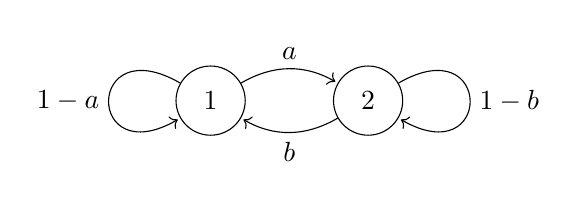
\begin{tikzpicture}[shorten >=1pt,node distance=2cm,on grid,auto] 
   \node[state] (q1)   {1}; 
   \node[state] (q2) [right=of q1] {2}; 
    \path[->] 
    (q1) edge[in=210, out=150] [loop] node[swap] {$1-a$} (q1)
    (q1) edge [bend left] node {$a$} (q2)
    (q2) edge[in=330, out=30] [loop] node {$1-b$} (q2)
    (q2) edge [bend left] node {$b$} (q1);
\end{tikzpicture}
\end{center}


Assume that $0 < a,b < 1$. We know from previous experience that
\[
    \pi = \begin{bmatrix}
        \frac{b}{a+b} & \frac{a}{a+b}
    \end{bmatrix}
\]

Now, let us consider this DTMC as a renewal process with renewals being visits to state $1$. Thus, $\mu$ denotes the mea return time to state $1$ and $N(t)$ captures the number of visits to state $1$ until time $t$. From the strong law of large numbers, we see that
\[
    \frac{N(t)}{t} \xrightarrow[a.s]{t \, \uparrow \, \infty} \frac{1}{\mu}
\]

Note, however, that by definition, the limit on the left is in fact the first element of the \emph{time-averaged distribution}, $\theta_1$. Thus, renewal theory tells us that
\[
    \theta_1 = \frac{1}{\mu}
\]
It is also easy to compute $\mu$. This is left as an exercise. It turns out that $\mu = \frac{a+b}{b} = \frac{1}{\pi_1}$. Hence, we get
\[
    \theta_1 = \frac{1}{\mu} = \pi_1
\]
Similar arguments also show that, $\theta_2 = \pi_2$. Thus, we see that
\[
    \theta = \pi = l
\]
That is, all three distributions of interest coincide. Thus, renewal theory helped us tackle the time-averaged distribution for the simple Gilbert-Elliot case. We shall see that on developing some more theory, we will be able to state and prove deeper and more general results. 

\subsection{The Inspection Paradox: Motivation}

We now develop the motivation for our next topic with the help of a famous probability riddle - the inspection paradox. Consider a renewal process where the renewals denote the arrival of buses at a bus stop. The question is as follows - you arrive at the bus stop at a random time. What is your average waiting time? Intuition would lead you to say $\frac{\mu}{2}$ since on an average you're somewhere in the middle of two arrivals. However, that is not correct. You are more likely to land in an interval of longer length and hence your average waiting time would be more than $\frac{\mu}{2}$. The precise answer really is that it depends on how the interarrival times are distributed. Note that we are now in the realm of continuous time. For argument's sake, suppose that $\mu = 10$ minutes. That is, the expectation of the interarrival times is fixed at $10$ minutes. It turns out that the following are true:
\begin{itemize}
    \item If the interarrival times are deterministic, then the expected waiting time is $5$ minutes
    \item If the interarrival times are exponential, then the expected waiting time is $10$ minutes (memorylessness?)
    \item If the interarrival times are degenerate hyperexponential ($0$ with probability $0.5$ and exponential with parameter $\frac{1}{20}$ with probability $0.5$) then the expected waiting time is $20$ minutes
\end{itemize}

Thus, there is no fixed answer to the `paradox'. We will soon show that the expected waiting time is equal to $5$ minutes only for the deterministic case and is greater than $5$ minutes for all other distributions. We will also find an explicit expression for the expected waiting time. 

A final note: Determinism is the best public policy! If passengers are arriving randomly at a bus stop, then the buses must determinstically arrive at fixed intervals for the expected waiting time to be minimised for the passengers. Any deviation from this would only increase the waiting time. 

\subsection{Renewal-Reward Theory}

On top of a renewal process, we may also add a \emph{reward signal}, most typically denoted by $R(t)$. This reward signal denotes the instantaneous `reward' at time $t$. We further assume that the value of $R(t)$ only depends on the present renewal cycle. Motivated by the bus stop example, we may define the reward signal to be the waiting time. The total reward accumulated in the $n^{\text{th}}$ renewal cycle is defined as
\[
    R_n \vcentcolon= \int_{S_{n-1}}^{S_n} \, R(s) \, ds
\]
with $S_0$ being defined as $0$. Further, we assume that $\left\{ (X_n, R_n) \right\}_{n \geq 1}$ are independent and $\left\{ (X_n, R_n) \right\}_{n \geq 2}$ are i.i.d.  Note that $X_n$ and $R_n$ may depend on each other. 

As a simple example, given a renewal process $N(t)$ with interarrival times $\left\{ X_i \right\}_{i \geq 1}$, define $R(t) \vcentcolon=$ time until next arrival. You should convince yourself that the following is true:
\[
    R(t) = S_{N(t)+1} - t
\]
The cumulative reward can then be calculated as
\[
    R_n = \frac{1}{2} X_n^2
\]
Now, $\left\{ (X_n, R_n) \right\}_{i \geq 1}$ defines a renewal-reward process. 
\begin{thm}[Renewal-Reward Theorem] \label{thm:rrt}
Given a renewal-reward process with reward signal $R$ and interarrival times $X_i$, we have
\[
    \frac{1}{t} \, \int_0^t \, R(s) \, ds \, \xrightarrow[a.s]{t \, \uparrow \, \infty} \, \frac{\mathbb{E} [ R_2 ]}{\mathbb{E}[X_2]}
\]
\end{thm}

We shall prove this theorem soon. Intuitively, it says that the long run time-averaged reward equals the expected reward in a cycle divided by the expected length of a cycle. Let us now apply this theorem to the inspection paradox. We have $R(t) = S_{N(t)+1} - t$ and $R_n = \frac{1}{2} X_n^2$. Thus, the expected waiting time is given by
\[
    \mathbb{E}[ \text{waiting time}] = \frac{\mathbb{E}[R_2]}{\mathbb{E}[X_2]} = \frac{1}{2} \frac{\mathbb{E}[X^2_2]}{\mathbb{E}[X_2]}
\]
Since we know $\mathbb{E}[X_2^2] \geq \left( \mathbb{E}[X_2] \right)^2$ with inequality only holding for the deterministic distribution, we immediately see that
\[
    \mathbb{E}[ \text{waiting time}] \geq \frac{\mu}{2}
\]
Thus, the expected waiting time is always greater than $\frac{\mu}{2}$ and it is equal to $\frac{\mu}{2}$ only when the distribution is deterministic, proving our earlier claim. Notice that for heavy-tailed distributions, it possible that the average interarrival time between buses is $10$ minutes and yet the average waiting time is infinity (when the second moment is infinity)!

\begin{proof}[Proof of Theorem \ref{thm:rrt}]
    Without loss of generality, we may assume the reward to be non-negative. If not, we can separate out the positive and negative parts of the reward and apply the following arguments to each part individually. The total reward accumulated upto time $t$ lies between the sum of the cumulative rewards of the first $N(t)$ renewal cycles and the first $N(t)+1$ renewal cycles (since the reward is non-negative). Hence, we have
    \[
        \frac{1}{t} \sum_{i=1}^{N(t)} R_i \leq \frac{1}{t} \int_0^t \, R(s) \, ds \leq \frac{1}{t} \sum_{i=1}^{N(t)+1} R_i
    \]
    \[
        \therefore \, \frac{N(t)}{t} \cdot \frac{1}{N(t)} \sum_{i=1}^{N(t)} R_i \leq \frac{1}{t} \int_0^t \, R(s) \, ds \leq \frac{N(t)+1}{t} \cdot \frac{1}{N(t)+1} \sum_{i=1}^{N(t)+1} R_i
    \]
    Letting $t \to \infty$ and on a trivial application of SLNN and Sandwich Theorem, we conclude that
    \[
        \frac{1}{t} \, \int_0^t \, R(s) \, ds \xrightarrow[a.s]{t \, \uparrow \, \infty} \frac{\mathbb{E}[R_2]}{\mathbb{E}[X_2]}
    \]
\end{proof}

Note that the reward need not be `continuous' and can be one-shot. That is, the entire cumulative reward for a renewal cycle can be received in one go at the start or end or at any point in the middle of the renewal cycle. In this case, the integral on the left hand side of Theorem \ref{thm:rrt} is not well-defined but as long as the integral on the left hand side is interpreted as the total reward accumulated upto time $t$, the theorem holds. Notice however that in the inspection paradox, we are not looking for a time-averaged waiting time as is prescribed by the Renewal-Reward Theorem. What we are really interested in, is $\mathbb{E}[R(t)]$. We have the following useful result for the same. 

\begin{thm} \label{thm:rrt_2}
    Suppose $\left\{ (X_n, R_n) \right\}_{n \geq 1}$ is a renewal-reward process and $\left\{ X_i \right\}_{i \geq 1}$ are non-arithmetic. Then, under mild regularity conditions, 
    \[
        \lim_{t \to \infty} \, \mathbb{E} \left[ R(t) \right] = \frac{\mathbb{E}[R_2]}{\mathbb{E}[X_2]}
    \]
\end{thm}

Rather than a time-averaged behaviour, this theorem talks about the limiting behaviour of the reward signal after a very long time. Notice that in this case, we need $R(t)$ to be well-defined and hence one-shot rewards are not possible.

\newpage

\section{Countable State-Space DTMCs}

\subsection{Classification of States}

We will now use our knowledge of renewal theory to generalise some of the ideas for finite DTMCs to countable DTMCs. We start off with some definitions. 
\[
    f_{ij}^{(n)} \vcentcolon= \P \left( X_n = j, X_k \neq j \text{ for } 1 \leq k \leq n-1 \mid X_0 = i \right)
\]
Intuitively, $f_{ij}^{(n)}$ is the probability that the first visit to state $j$ starting at state $i$ occurs in $n$ steps. Notice that $f_{ij}^{(n)} \leq p_{ij}^{(n)}$. We also define
\[
    f_{ij} \vcentcolon= \sum_{n=1}^{\infty} f_{ij}^{(n)}
\]
$f_ij$ is the probability of ever hitting state $j$ starting at state $i$. If $f_{ij} < 1$, then there is a positive probability of never reaching state $j$ starting from state $i$. If $f_{ij} = 1$ then the DTMC will hit state $j$ starting from state $i$ with probability $1$. In the second case, it is meaningful to define another random variable, $T_{ij}$ which is the hitting time of state $j$ starting at state $i$. When $f_{ij} = 1$, $f_{ij}^{(n)}$ describes the p.m.f of $T_{ij}$. Moreover, we define
\[
    \nu_{ij} \vcentcolon= \mathbb{E} \left[ T_{ij} \right] = \sum_{n=1}^{\infty} n \cdot f_{ij}^{(n)}
\]
$\nu_{ij}$ is the expected hitting time of state $j$ starting at state $i$. We classify the states of a DTMC as follows. 

\begin{defn} [Classification of States]
    Given a DTMC, a state $i$ is said to be \emph{transient} if $f_{ii} < 1$ and is said to be \emph{recurrent} if $f_{ii} = 1$. A recurrent state is further classified as \emph{null-recurrent} if $\nu_{ii} = \infty$ and \emph{positive-recurrent} if $\nu_{ii} < \infty$.
\end{defn}

We will also be interested in knowing the mean number of returns to a state. For this purpose, we define
\[
    M_i \vcentcolon= \sum_{k=1}^{\infty} \mathbbm{1}_{\left\{X_k = i  \right\}}
\]
$M_i$ denotes the number of visits to state $i$. The expected number of returns to state $i$, starting from state $i$ is then given by
\begin{align*}
    \mathbb{E}\left[ \, M_i \mid X_0 = i \, \right] &= \mathbb{E} \left[ \sum_{k=1}^{\infty} \mathbbm{1}_{\left\{ X_k = i \right\}} \mid X_0 = i \right] \\
    &= \sum_{k=1}^{\infty} \mathbb{E} \left[ \mathbbm{1}_{\left\{X_k = i \right\}} \mid X_0 = i \right] \\
    &= \sum_{k=1}^{\infty} \P \left( X_k = i \mid X_0 = i \right)
\end{align*}
\[
    \therefore \, \mathbb{E} \left[ \, M_i \mid X_0 = i \, \right] = \sum_{k=1}^{\infty} p_{ii}^{(k)}
\]

\begin{lem}
    For a transient state $i$, with $X_0 = i$, the number of returns to $i$ is finite with probability $1$. Further, the expected number of returns is also finite and thus
    \[
        \sum_{k=1}^{\infty} p_{ii}^{(k)} < \infty
    \]
\end{lem}

\begin{proof}
    The proof of the above Lemma follows rather trivially by observing that the probability of the number of returns being $k$ is given by $f_{ii}^{k} \cdot \left( 1 - f_{ii} \right)$. This is a shifted geometric distribution and hence, the number of returns is finite with probability $1$. Further, the expectation is given by
    \[
        \frac{f_{ii}}{1 - f_{ii}}
    \]
    which is finite for transient states since $f_{ii} < 1$. 
\end{proof}

We have a similar lemma for recurrent states. As expected, the number of returns turns out to be infinite. Interestingly, if we look at the limit of the time-averaged number of returns, that helps us classify recurrent states into positive or null. This is formalised below.

\newpage

\begin{lem}
    For a recurrent state $i$, with $X_0 = i$, the number of returns to $i$ is infinite with probability $1$. The expected number of returns is also infinite and thus
    \[
        \sum_{k=1}^{\infty} p_{ii}^{(k)} = \infty
    \]
    Further, we have
    \[
        \lim_{n \to \infty} \, \frac{1}{n} \sum_{k=1}^{n} p_{ii}^{(k)} = \begin{cases}
            0 & \text{ if $i$ is null-recurrent} \\
            \frac{1}{\nu_{ii}} & \text{ if $i$ is positive-recurrent}
        \end{cases}
    \]
\end{lem}

\begin{proof}
    We define a renewal process with $S_n$ denoting the time of the $n^{\text{th}}$ return to state $i$ with $X_0 = i$. $\left\{ S_n \right\}_{n \geq 1}$ are i.i.d with mean $\nu_{ii}$. Note that this renewal process is only well-defined because interarrival times are finite with probability $1$. Then, $N(n)$ is the number of returns to state $i$ by time $n$ and $m(n)$ is the expected number of returns to state $i$ by time $n$. Formally, we have
    \[
        N(n) = \sum_{k=1}^{n} \mathbbm{1}_{\left\{X_k = i \right\}}
    \]
    and
    \[
        m(n) = \sum_{i=1}^{n} p_{ii}^{(k)}
    \]
    By statements $1$ and $2$ of Lemma \ref{lem:ren_1}, we immediately get
    \begin{align*}
        N(n) &\xrightarrow[a.s]{n \, \uparrow \, \infty} \infty \\
        m(n) &\xrightarrow[]{n \, \uparrow \, \infty} \infty
    \end{align*}
    
    By applying the elementary renewal theorem (Theorem \ref{thm:elementary}), we get
    \[
        \frac{m(n)}{n} \xrightarrow[]{n \, \uparrow \, \infty} \frac{1}{\mu}
    \]
    Note that for $\mu = \infty$, we interpret the right hand side as $0$. Thus, the third statement of the lemma follows trivially. 
\end{proof}

\newpage

To summarise, we have the following equivalences:

\begin{align*}
    i \text{ is transient } &\iff \, \sum_{k=1}^{\infty} p_{ii}^{(k)} < \infty \\
    i \text{ is null-recurrent } &\iff \, \sum_{k=1}^{\infty} p_{ii}^{(k)} = \infty \text{  and } \lim_{n \to \infty} \, \frac{1}{n} \sum_{k=1}^{\infty} p_{ii}^{(k)} = 0 \\
    i \text{ is positive-recurrent } &\iff \, \sum_{k=1}^{\infty} p_{ii}^{(k)} = \infty \text{  and } \lim_{n \to \infty} \, \frac{1}{n} \sum_{k=1}^{\infty} p_{ii}^{(k)} > 0
\end{align*}

For irreducible DTMCs, we have the following remarkable theorem. 

\begin{thm} \label{thm:irreducible-states}
    All states of an irreducible DTMC are of the same type - transient or null-recurrent or positive-recurrent. In this case, we call the entire DTMC transient or null-recurrent or positive-recurrent.
\end{thm}

\setcounter{equation}{0}

\begin{proof}
    Pick any two states $i,j \in S$ with $i \neq j$. By irreducibility, $\exists \, r,s \in \mathbb{N}$ such that $p_{ji}^{(r)} > 0$ and $p_{ij}^{(s)} > 0$, We have
    \[
        p_{jj}^{(r+s+k)} \geq p_{ji}^{(r)} \cdot p_{ii}^{(k)} \cdot p_{ij}^{(s)}
    \]
    Summing with respect to $k$, we get
    \[
        \sum_{k=1}^{n} p_{jj}^{(r+s+k)} \geq p_{ji}^{(r)} \cdot p_{ij}^{(s)} \cdot \sum_{k=1}^n p_{ii}^{(k)}
    \]
    We may further write
    \begin{align}
        \sum_{k=1}^{r+s+n} p_{jj}^{(k)} &\geq p_{ji}^{(r)} \cdot p_{ij}^{(s)} \cdot \sum_{k=1}^n p_{ii}^{(k)}
    \end{align}
    
    Now, suppose $j$ is transient. Then, taking limits on both sides, we have
    \[
        \infty > \, \sum_{k=1}^{\infty} p_{jj}^{(k)} \, \geq p_{ji}^{(r)} \cdot p_{ij}^{(s)} \cdot \sum_{k=1}^{\infty} p_{ii}^{(k)} \implies \sum_{k=1}^{\infty} p_{ii}^{(k)} < \infty
    \]
    Thus, the transience of $j$ implies the transience of $i$. But $i,j$ were arbitrary. Hence, if any one state is transient then all others are transient. 
    
    \medskip
    
    Suppose $j$ is null-recurrent. From equation $(1)$, we have
    \[
        \frac{1}{n} \, \sum_{k=1}^{r+s+n} p_{jj}^{(k)} \, \geq \, p_{ji}^{(r)} \cdot p_{ij}^{(s)} \cdot \left( \frac{1}{n} \, \sum_{k=1}^n p_{ii}^{(k)} \right)
    \]
    As $n \to \infty$, the LHS has a limit of zero. Hence, we get
    \[
        \limsup_{n \to \infty} \, \frac{1}{n} \, \sum_{k=1}^n p_{ii}^{(k)} \leq 0
    \]
    Since the above sequence is non-negative, we have
    \[
        \lim_{n \to \infty} \, \frac{1}{n} \, \sum_{k=1}^n p_{ii}^{(k)} = 0
    \]
    Since $j$ is not transient, $i$ cannot be transient either. Hence, $i$ must be null-recurrent. Thus, if one state is null-recurrent, all states are null-recurrent. The proof for positive-recurrent follows rather trivially from the above two parts on noting that a state can be only one of three - transient, null-recurrent or positive-recurrent.
\end{proof}

Thus, to summarise, we have three kinds of irreducible DTMCs - transient chains, null-recurrent chains and positive-recurrent chains.

\newpage

\subsection{Transient Chains}

We now begin studying transient chains. It turns out that there is no meaningful long-run behaviour for transient chains, hence they are of no practical importance to us. Nonetheless, we will formalise the long-run behaviour of transient chains for the sake of completeness. 

\begin{thm} \label{thm:transient_long_run}
    For an irreducible, transient chain, the following hold true
    
    \begin{enumerate}
        \item For any $j \in S$, 
        \[
            \sum_{k=1}^{\infty} \mathbbm{1}_{\left\{ X_k = j \right\}} < \infty \quad \text{almost surely}
        \]
        Thus, there is no time-averaged distribution for irreducible transient chains.
        
        \item For any $i,j \in S$, we have
        \[
            \sum_{k=1}^{\infty} p_{ij}^{(k)} < \infty
        \]
        
        \item \[
            \lim_{k \to \infty} \, p_{ij}^{(k)} = 0 \quad \forall \, i,j \in S
        \]
        Hence, there is no limiting distribution for irreducible transient chains. 
        
        \item There is no stationary distribution.
    \end{enumerate}
\end{thm}

As we see, there is no meaningful long-run behaviour for transient chains. 

\begin{proof}
    \begin{enumerate}
        \item Let $M_j$ be the number of visits to state $j$ over time $k \geq 1$ and let $p_j$ be the probability of once reaching $j$ after time $0$. Then, we have
        \[
            \P \left( M_j = 0 \right) = 1- p_j
        \]
        \[
            \P \left( M_j = k \right) = p_j \cdot f_{ii}^{k-1} \cdot (1 -f_{ii})
        \]
        Since this is a valid, non-degenerate p.m.f, we see that $M_j$ is finite with probability $1$.
        
        \item Let $X_0 = i$. From the above p.m.f, we have $\mathbb{E} \left[ M_j \right] < \infty$. But, we see that 
        \[
            \mathbb{E} \left[ M_j \right] = \sum_{k=1}^{\infty} p_{ij}^{(k)}
        \]
        Thus, the second result follows.
        
        \item Follows from 2. 
        
        \item Pick some state $i \in S$. We have
        \[
            \P \left( X_n = i \right) = \mu_n(i) = \sum_{j \in S} \mu_0(j) \cdot p_{ji}^{(n)}
        \]
        Taking limits on both sides, we get
        \[
            \lim_{n \to \infty} \mu_n(i) = \lim_{n \to \infty} \sum_{j \in S} \mu_0(j) \cdot p_{ji}^{(n)}
        \]
        By the Dominated Convergence Theorem, we may switch the limit with the summation. Hence, we get
        \[
            \lim_{n \to \infty} \mu_n(i) = \sum_{j \in S} \mu_0(j) \cdot \lim_{n \to \infty} p_{ij}^{(n)} 
        \]
        \[
            \therefore \, \lim_{n \to \infty} \mu_n(i) = 0 \quad \forall \, i \in S
        \]
        Suppose a stationary distribution $\pi$ existed. Then, $\exists \, i \in S$ such that $\pi_i > 0$. Suppose further that $\mu_0 = \pi$. Then $\mu_n = \pi$ for all $n$, by virtue of stationarity. Thus, $\mu_n(i) = \pi_i > 0$ for all $n$, however this contradicts $\lim_{n \to \infty} \mu_n(i) = 0$. Thus, no stationary distribution can exist.
    \end{enumerate}
\end{proof}

A common example of a transient chain is what is known as the \emph{Drunkard's Random Walk}, which is a random walk on $\mathbb{Z}$. Starting at $0$, at every time step, the drunkard moves right with probability $p$ and left with probability $q = 1-p$. The behaviour of this chain is characterised by
\[
    \sum_{n=1}^{\infty} p_{00}^{(n)} 
\]
Since the drunkard may return to state $0$ only after an even number of steps, we shall look at 
\[
    \sum_{n=1}^{\infty} p_{00}^{(2n)}
\]

Also note that we have
\[
    p_{00}^{(2n)} = \binom{2n}{n} \cdot p^n \cdot q^n
\]

We will make use of \emph{asymptotic notation}. Namely, we have the following notation
\[
    f(n) \sim g(n) \iff \lim_{n \to \infty} \frac{f(n)}{g(n)} = 1
\]
We will also make use of Stirling's approximation of the factorial, that is
\[
    n! \sim \left( \frac{n}{e} \right)^n \sqrt{2\pi n}
\]
Thus, we get
\[
    p_{00}^{(2n)} \sim \frac{\left( 4pq \right)^n}{\sqrt{\pi n}}
\]

We will now consider two cases. 

\medskip

\underline{Case 1}: $p \neq q$. This is a biased random walk. We have
\[
    pq < \frac{1}{4} \iff 4pq < 1
\]
Thus, we have
\[
    p_{00}^{(2n)} \sim \frac{a^n}{\sqrt{\pi n}} 
\]
with $a \in (0,1)$. Given any $\epsilon > 0$, there exists $n_0 \in \mathbb{N}$ such that
\[
    (1- \epsilon) \cdot \frac{a^n}{\sqrt{\pi n}} \leq \, p_{00}^{(2n)} \, \leq (1+\epsilon) \cdot \frac{a^n}{\sqrt{\pi n}} \quad \forall \, n \geq n_0
\]
Now, 
\[
    \sum_{n=1}^{\infty} p_{00}^{(2n)} = \sum_{n=1}^{n_0 - 1} p_{00}^{(2n)} + \sum_{n=n_0}^{\infty} p_{00}^{(2n)} < \infty
\]
Thus, the chain is transient.

\medskip

\underline{Case 2}: $p = q = \frac{1}{2}$. This is an unbiased random walk. We have
\[
    pq = \frac{1}{4} \iff 4pq = 1
\]
Thus, 
\[
    p_{00}^{(2n)} \sim \frac{1}{\sqrt{\pi n}}
\]
We immediately see that 
\[
    \sum_{n=1}^{\infty} p_{00}^{(2n)} = \infty
\]
Hence, the chain is recurrent. Similar to the first case, given any $\epsilon > 0$, there exists $n_0 \in \mathbb{N}$ such that
\[
    \frac{1-\epsilon}{\sqrt{\pi n}} \leq \, p_{00}^{(2n)} \, \leq \frac{1+\epsilon}{\sqrt{\pi n}} \quad \forall \, n \geq n_0
\]
Thus, we have
\[
    \frac{1}{2n} \sum_{k=1}^{\infty} p_{00}^{(2k)} \leq \frac{1}{2n} \sum_{k=1}^{n_0-1} p_{00}^{(2k)} + \frac{1+\epsilon}{2n} \sum_{k=n_0}^{n} \frac{1}{\sqrt{\pi n}}
\]
Letting $n \to \infty$, we see that
\[
    \limsup_{n \to \infty} \, \frac{1}{2n} \sum_{k=1}^{n} p_{00}^{(2k)} \leq 0 
\]
and hence,
\[
    \lim_{n \to \infty} \, \frac{1}{2n} \sum_{k=1}^n p_{00}^{(2k)} = 0
\]
Hence, the chain is null-recurrent.

\subsection{Recurrent Chains}

We now talk about recurrent chains. The first result we prove is that in an irreducible recurrent chain, every state is visited with probability $1$ regardless of the starting state.

\begin{lem} \label{lem:fij_equals_1}
    In an irreducible, recurrent chain, 
    \[
        f_{ij} = 1 \quad \forall \, i,j \in S
    \]
\end{lem}

\begin{proof}
    We prove this by contradiction. Suppose $f_{ij} < 1$ and suppose $X_0 = j$. With some positive probability, $p$, the chain visits state $i$ before returning to state $j$. Hence, with probability $p(1-f_{ij})$, the chain never returns to $j$. This contradicts $f_{jj} = 1$.
\end{proof}

The next theorem talks about the long-run behaviour of recurrent chains. We will later show that this theorem tells us that for null-recurrent chains, no meaningful long-run behaviour exists.

\begin{thm} \label{thm:recurrent_long_run}
    Consider an irreducible recurrent chain. For any $j \in S$, we define
    \[
        M_j(n) \vcentcolon= \sum_{k=1}^{n} \mathbbm{1}_{\left\{ X_k = j \right\}}
    \]
    $M_j(n)$ counts the number of visits to state $j$ after time $0$ and up to time $n$. Then, we have
    \begin{enumerate}
        \item \[
            \frac{M_j(n)}{n} \xrightarrow[a.s]{n \, \uparrow \, \infty} \frac{1}{\nu_{jj}}
        \]  
        \item 
        \[
            \frac{\mathbb{E} \left[ M_j(n) \mid X_0 = i \right]}{n} = \frac{1}{n} \sum_{k=1}^{n} p_{ij}^{(k)} \xrightarrow[]{n \, \uparrow \, \infty} \frac{1}{\nu_{jj}}
        \]
        \item If the chain is aperiodic, then
        \[
            p_{ij}^{(n)} \xrightarrow[]{n \, \uparrow \, \infty} \frac{1}{\nu_{jj}}
        \]
    \end{enumerate}
\end{thm}

An immediate corollary of Theorem \ref{thm:recurrent_long_run} when specialised to null-recurrent and positive-recurrent chains, is that for null-recurrent chains, there is no time-averaged distribution. If also aperiodic, there is no limiting distribution either. For aperiodic, irreducible, positive-recurrent chains, a meaningful time-averaged distribution and limiting distribution exists so long as
\[
    \sum_{j} \frac{1}{\nu_{jj}} = 1
\]
We will soon prove that this is indeed the case. 

\begin{proof}
    \begin{enumerate}
        \item Define a renewal process with renewals at visits to state $j$ after time $0$. Let $\left\{ Y_i \right\}$ denote the inter-renewal times. By Lemma \ref{lem:fij_equals_1}, $Y_1$ is finite with probability $1$. Further, $\left\{ Y_i \right\}_{i \geq 2}$ are i.i.d with mean $\nu_{jj}$. A trivial application of SLNN for renewal processes (Theorem \ref{thm:slnn}) gives us
        \[
            \frac{M_j(n)}{n} \xrightarrow[a.s]{n \, \uparrow \, \infty} \frac{1}{\nu_{jj}}
        \]
        
        \item Consider the same renewal process as above specialised with $X_0 = i$. Then, the the numerator of the RHS is the expected number of renewals up to time $n$. Thus, the statement follows by the Elementary Renewal Theorem (Theorem \ref{thm:elementary}).
        
        \item Consider the same renewal process as before. $\left\{ Y_i \right\}_{i \geq 2}$ are arithmetic with span $d_j^{\prime} \vcentcolon= \gcd\left\{ n \colon f_{jj}^{(n)} > 0 \right\}$. Let $d_j \vcentcolon= \gcd\left\{ n \colon p_{jj}^{(n)} > 0 \right\}$. By aperiodicity, $d_j = 1$. In Lemma \ref{lem:gcd_p_equals_gcd_f}, which shortly follows the proof of this theorem, we show that $d_j^{\prime} = d_j$. Hence, by application of Blackwell's Renewal Theorem (Theorem \ref{thm:brt}), we see that
        \[
            \lim_{n \to \infty} p_{ij}^{(n)} = \frac{1}{\nu_{jj}}
        \]
    \end{enumerate}
\end{proof}

\begin{lem} \label{lem:gcd_p_equals_gcd_f}
    For any state $j \in S$, let $N_j \vcentcolon= \left\{ n \colon p_{jj}^{(n)} > 0 \right\}$ and $N_j^{\prime} \vcentcolon= \left\{ n \colon f_{jj}^{(n)} > 0 \right\}$. Then, $\gcd(N_j) = \gcd(N_j^{\prime})$. 
\end{lem}

\begin{proof}
    Let $d_j \vcentcolon= \gcd(N_j)$ and $d_j^{\prime} \vcentcolon= \gcd(N_j^{\prime})$. We know that $f_{jj}^{(n)} \leq p_{jj}^{(n)}$. Hence, $N_j^{\prime} \subseteq N_j$. Thus, $d_j^{\prime} \geq d_j$. Further, any element of $N_j$ is a sum of elements of $N_j^{\prime}$. Hence, $d_j^{\prime}$ divides every element of $N_j$. Thus, $d_j^{\prime} \leq d_j$. Hence, $d_j = d_j^{\prime}$.
\end{proof}


\begin{lem} \label{lem:finite_irreducible_positive}
    Any finite, irreducible DTMC is necessarily positive-recurrent.
\end{lem}

\begin{proof}
    Let $S$ be the state-space of the DTMC. $S$ is finite. As done before, we define
    \[
        M_j(n) \vcentcolon= \sum_{k=1}^{n} \mathbbm{1}_{\left\{ X_k = j \right\}}
    \]  
    Observe that
    \[
        \sum_{j \, \in \, S} M_j(n) = n \quad \forall \, n \in \mathbb{N}
    \]
    Hence, we get
    \[
        \lim_{n \to \infty} \, \frac{1}{n} \sum_{j \, \in \, S} M_j(n) = 1 
    \]  
    Since the first summation is finite, we may exchange the limit with the summation. Thus, we get
    \[
        \sum_{j \, \in \, S} \lim_{n \to \infty} \frac{M_j(n)}{n} = 1
    \]
    Now, suppose that the chain was either transient or null-recurrent. Theorems \ref{thm:transient_long_run} and \ref{thm:recurrent_long_run} tell us that for both cases
    \[
        \frac{M_j(n)}{n} \xrightarrow[a.s]{n \, \uparrow \, \infty} 0 \quad \forall \, j \in S
    \]
    Hence, this violates the condition we laid out before since a finite number of zeroes cannot possibly add up to $1$. Hence, the chain must be positive-recurrent.
\end{proof}

Now, we lay down the `big' theorem which completely characterises the long-run behaviour of positive-recurrent chains.

\begin{thm}
    An irreducible DTMC is positive-recurrent if and only if there exists a probability distribution $\pi$ such that $\pi = \pi \cdot P$. Such a $\pi$ is unique, element-wise positive and
    \[
        \pi_i = \frac{1}{\nu_{ii}}
    \]  
\end{thm}

\begin{proof}
    Since this is an if and only if statement, we must prove both implications. We first prove the backward implication. Suppose there exists a stationary distribution $\pi$. By Lemma \ref{lem:stat_positive}, $\pi > 0$, entry-wise. Also, the chain is necessarily recurrent since transient chains don't have a stationary distribution. Consider the DTMC with $\mu_0 = \pi$. Using the same definition for $M_j(n)$ as before, we get
    \[
        \mathbb{E} \left[ M_j(n) \right] = n \cdot \pi_j \implies \frac{1}{n} \mathbb{E} \left[ M_j(n) \right] = \pi_j
    \]
    Thus, we also have
    \[
        \lim_{n \to \infty} \frac{1}{n} \mathbb{E} \left[ M_j(n) \right] = \pi_j
    \]
    We also have
    \[
        \frac{1}{n} \mathbb{E} \left[ M_j(n) \right] = \sum_{i \, \in \, S} \frac{1}{n} \mathbb{E} \left[ M_j(n) \mid X_0 = i \right] \cdot \pi_i = \sum_{i \, \in \, S} \pi_i \cdot \left( \frac{1}{n} \sum_{k=1}^{n} p_{ij}^{(k)} \right)
    \]
    We now take limit $n \to \infty$. An application of the Dominated Convergence Theorem allows us to switch the sum with the limit. Thus, we have
    \[
        \lim_{n \to \infty} \frac{1}{n} \mathbb{E} \left[ M_j(n) \right] = \sum_{i \, \in S} \pi_i \cdot \lim_{n \to \infty} \left( \frac{1}{n} \sum_{k=1}^n p_{ij}^{(k)} \right) = \sum_{i \, \in \, S} \pi_i \cdot \frac{1}{\nu_{jj}} = \frac{1}{\nu_{jj}}
    \]
    
    Hence, we get
    \[
        \pi_j = \frac{1}{\nu_{jj}}
    \]
    Since, $\pi_j > 0$, we have $\nu_{jj} < \infty$. Thus, the chain is positive-recurrent. Since $\nu_{jj}$ is unique, the stationary distribution is also unique. This concludes the proof for the backward implication.
    
    \medskip
    
    Suppose now that the chain is positive-recurrent. We have to show that there exists a stationary distribution. Define a vector
    \[
        \pi = \left( \frac{1}{\nu_{jj}} \, , \, j \in S \right)
    \]
    At this point, this is just a vector and not necessarily a distribution (it will turn out to be one). $\pi > 0$ since $\nu_{jj}$ is finite. Let $a^{(n)}$ denote the first row of $\frac{1}{n} \sum_{k=1}^n P^k$ and let $b^{(n)}$ denote the first row of $\frac{1}{n} \sum_{k=2}^{n+1} P^k$. By definition, we see that $b^{(n)} = a^{(n)} \cdot P$. Also, 
    \[
        a_j^{(n)} = \frac{1}{n} \sum_{k=1}^{n} p_{1j}^{(k)}
    \]
    Thus, $a^{(n)}_j \xrightarrow[]{n \, \uparrow \, \infty} \pi_j$. Similarly, we have $b^{(n)}_j \xrightarrow[]{n \, \uparrow \, \infty} \pi_j$. we have
    \[
        b_j^{(n)} = \sum_i a_i^{(n)} p_{ij} \geq \sum_{i=1}^M a_i^{(n)} p_{ij}
    \]
    Letting $n$ go to $\infty$, we have
    \[
        \pi_j \geq \sum_{i=1}^M \pi_i \cdot p_{ij}
    \]
    Now letting, $M$ go to $\infty$, we have
    \[
        \pi_j \geq \underbrace{\sum_{i=1}^{\infty} \pi_i \cdot p_{ij}}_{\beta_j} \implies \pi_j \geq \beta_j \quad \forall \, j \in S
    \]
    Note that
    \[
        \sum_{j \, \in \, S} a_j^{(n)} = 1 \implies \sum_{j=1}^M a_j^{(n)} \leq 1
    \]
    Letting $n$ go to $\infty$, we get
    \[
        \sum_{j=1}^M \pi_j \leq 1
    \]
    Letting $M$ go to $\infty$, we see that
    \[
        \sum_{j=1}^{\infty} \pi_j \leq 1
    \]
    Hence, $\pi$ is summable. Summing $\beta_j$ over all $j$, we get
    \[
        \sum_{j} \beta_j = \sum_j \sum_i \pi_i \cdot p_{ij} = \sum_i \pi_i \sum_j p_{ij} = \underbrace{\sum_i \pi_i}){\alpha}
    \]
    Thus, we have
    \[
        \sum_j \pi_j = \sum_j \beta_j \quad \text{and} \quad \pi_j \geq \beta_j \quad \forall \, j \in S
    \]
    This gives us that
    \[
        \pi_j = \beta_j \quad \forall \, j \in S \implies \pi = \pi \cdot P
    \]
    Thus, $\frac{\pi}{\alpha}$ is a stationary distribution. In conjunction with part $1$, we can also conclude that $\alpha = 1$ and hence $\pi$ itself is a stationary distribution.
\end{proof}

To summarise, for irreducible positive-recurrent chains, we have a unique stationary distribution, $\pi$. Moreover, the time-averaged distribution, $\theta$, exists and $\theta = \pi$. If the chain is also aperiodic, then there exists a limiting distribution $l$ and $l = \theta = \pi$. Thus, we have managed to completely characterise the long-run behaviour of every kind of irreducible DTMC. 

\medskip

We now take an interesting look at stationarity and time-reversibility through renewal-reward theory. 

\begin{lem} \label{lem:long_run_transition_rate}
    Consider an irreducible positive-recurrent DTMC. For any $i,j \in S$, the long-run rate of $i \to j$ transitions equals $\pi_i \cdot p_{ij}$. 
\end{lem}

\begin{proof}
    Define a renewal process where renewals are visits to state $i$ and the reward is $1$ if the immediate next state is $j$ and $0$ otherwise. Then, the number of $i \to j$ transitions up to time $n$ is exactly equal to the reward accumulated till time $n$. The expected reward in a single cycle is $p_{ij}$. The expected length of a renewal cycle is $\nu_{ii}$. Let $M_{ij}(n)$ be the number of $i \to j$ transitions up to time $n$. Thus, Renewal-Reward Theorem (Theorem \ref{thm:rrt}) tells us that
    \[
        \frac{M_{ij}(n)}{n} \, \xrightarrow[a.s]{n \, \uparrow \, \infty} \, \frac{p_{ij}}{\nu_{ii}} = \pi_i \cdot p_{ij}
    \]
    \end{proof}
    
    Using Lemma \ref{lem:long_run_transition_rate}, let us see a different interpretation of stationarity. We have
    \[
        \pi_i = \sum_j \pi_j \cdot p_{ji} \implies \sum_i \pi_i \cdot p_{ij} = \sum_j \pi_j \cdot p_{ji}
    \]

    The second equation simply states that the rate of exiting state $i$ is equal to the rate of entering state $i$. This is a very intuitive interpretation of the stationarity equations. The key thing to note is that the rate of exiting state $i$ and entering state $i$ from each state need not be equal. Only the total rate of exiting and entering state $i$ must balance. If we also have that every rate individually balances, the chain is time-reversible! Thus, time-reversibility may be re-interpreted as the rates of $i \to j$ transitions being equal to $j \to i$ transitions for all $i,j \in S$. Thus, stationarity talks about a global balance whereas time-reversibility talks about a finer local balance.
    
    \medskip
    
    So far, the only method we know to establish the positive recurrence is to look for the existence of a stationary distribution. Another interesting method to establish the positive recurrence of an irreducible chain is through \emph{Lyapunov Stability Analysis}, which is characterised by the following theorem. 
    
    \begin{thm}[Foster-Lyapunov Theorem]
        Consider an irreducible DTMC over a countable state space $S$. Suppose $V \colon S \to \mathbb{R}_+$ and $C$ is a finite subset of $S$. If there exists $\epsilon > 0$ and $b < \infty$ such that
        \begin{enumerate}
            \item $\mathbb{E} \left[ V(X_{k+1}) - V(X_k) \mid X_k = i \right] \leq -\epsilon \quad \forall \, i \in S \setminus C$
            \item $\mathbb{E} \left[ V(X_{k+1}) - V(X_k) \mid X_k = i \right] \leq b \quad \forall \, i \in C$
        \end{enumerate}
        then, the DTMC is positive recurrent.
    \end{thm}
    
    $V$ is called a \emph{Lyapunov} function. This theorem says that the DTMC is positive recurrent if the expected `drift' of the Lyapunov function is sufficiently negative for all but finitely many states and is finite for those finitely many states.
    
    \medskip
    
    We will consider another interesting application of Lyapunov stability, concerned with routing incoming packets to two different queues. We will consider the arrival of incoming packets to be $BP(a)$ and the service at the two queues to be $BP(d_1)$ and $BP(d_2)$. It is easy to show that we must have $a < d_1 + d_2$ for stability. Given that we have $a < d_1 + d_2$, how do we stabilise the system? A simple policy is to choose $p$ such that $ap < d_1$ and $a(1-p) < d_2$ and route each job to queue $1$ with probability $p$ and to queue $2$ with probability $(1-p)$.  One drawback about this policy is that it may turn out to be inefficient. For example, one queue may have a hundred jobs lined up while the other is empty and yet we may route a new job to the first queue. Another drawback is that we require the knowledge of $a, d_1, d_2$ to determine the policy, while this may not be available.
    
    \medskip
    
    A rather simple but effective policy, is to route the job to the shortest queue. We will show that this simple policy stabilises the system. Formally, we will let $X_i$ be the number of jobs waiting at queue $i$. We will consider our states to be $(X_1, X_2) \in \mathbb{Z}_+^2$. We will route the new job to queue $1$ if $X_1 \leq X_2$ and to queue $2$ if $X_1 > X_2$. Proving the positive recurrence of this chain (and stability of the system) by finding the stationary distribution is quite hopeless. Instead, we will use a Lyapunov approach. We define the Lyapunov function as 
    \[
        V(X) \vcentcolon= \frac{X_1^2 + X_2^2}{2}
    \]
    The update equations are as follows:
    \[
    X_i(t+1) = X_i(t) + A_i(t) - D_i(t) + L_i(t)
    \]
    where
    \[
        A_1(t) = A(t) \cdot \mathbbm{1}_{\left\{X_1 \leq X_2\right\}} \quad ; \quad A_2(t) = A(t) \cdot \mathbbm{1}_{\left\{X_1 > X_2\right\}}
    \]
    with $A(t) \sim BP(a)$. We also have $D_i(t) \sim BP(d_i)$. The term $L_i(t)$ is a correction term to disallow departures when the queue is empty. We have
    \[
        L_i(t) = \mathbbm{1}_{\left\{X_i(t) + A_i(t) - D_i(t) = -1\right\}}
    \]
    
    We then have
    \begin{align*}
        \Delta(X) &\vcentcolon= \mathbb{E} \left[ V(X(k+1)) - V(X(k)) \mid X(k) = x \right] \\
        &= \frac{1}{2} \sum_{i=1}^2 \mathbb{E} \left[ X_i^2(k+1) - X_i^2(k) \mid X(k) = x \right] \\
        &= \frac{1}{2} \sum_{i=1}^2 \mathbb{E} \left[ \left( X_i + A_i - D_i + L_i \right)^2 - X_i^2 \mid X = x \right] \\
        &\leq \frac{1}{2} \sum_{i=1}^2 \mathbb{E} \left[ \left( X_i + A_i - D_i \right)^2 - X_i^2(k) \mid X(k) = x \right] \\
        &= \frac{1}{2} \sum_{i=1}^2 \mathbb{E} \left[ 2 \cdot X_i \cdot (A_i - D_i) + \underbrace{\left(A_i - D_i\right)^2}_{\leq 1} \mid X(k) = x \right] \\
        &\leq 1 + \sum_{i=1}^2 \mathbb{E} \left[ X_i \cdot \left( A_i - D_i \right) \mid X(k) = x \right] \\
        &= 1 + X_1 \cdot \left( a \cdot \mathbbm{1}_{\left\{ X_1 \leq X_2 \right\}} \right) - X_1 D_1 + X_2 \cdot \left( a \cdot \mathbbm{1}_{\left\{ X_1 > X_2 \right\}} \right) - X_2 D_2
    \end{align*}
    Thus, we get
    \[
        \Delta(X) \leq 1 + a \cdot \min\left( X_1, X_2 \right) - X_1 D_1 -  X_2 D_2
    \]
    Now, we pick $p \in (0,1)$ such that $ap < d_1$ and $a(1-p) < d_2$ (this is possible since $a < d_1 + d_2$). Thus, we get
    \begin{align*}
        \Delta(X) &\leq 1 + a \cdot a \left( pX_1 + (1-p)X_2 \right) - X_1D_1 - X_2D_2 \\
        &= 1 + \underbrace{(ap-d_1}_{< 0} + \underbrace{\left( a(1-p) - d_2 \right)}_{<0}
    \end{align*}
    
    Now, for an $\epsilon > 0$, it suffices to have
    \[
        X_1 \geq \frac{1+\epsilon}{d_1 - ap} \quad \text{or} \quad X_2 \geq \frac{1+\epsilon}{d_2 - a(1-p)}
    \]
    to make $\Delta(X) \leq -\epsilon$. Thus if we choose
    \[
        C \vcentcolon= \left\{ (x_1, x_2) \in \mathbb{Z}_+^2 \mid 0 \leq x_1 \leq \left\lceil \frac{1+\epsilon}{d_1 - ap} \right\rceil \text{ and } 0 \leq x_2 \leq \left\lceil \frac{1+\epsilon}{d_2 - a(1-p)} \right\rceil \right\}
    \]
    Then, we have $\Delta(x) \leq -\epsilon$ for all $x \in S \setminus C$. Thus, by the Foster-Lyapunov Theorem, the chain is recurrent and hence the system is stable.
    
    \newpage
    
    \section{Exponential Distributions and Poisson Processes}
    
    Before moving on to continuous time Markov chains, we will review some properties about the exponential distribution and Poisson processes. 
    
    \begin{defn}[Exponential Random Variable]
        A random variable $X$ is said to be \emph{exponential} with parameter $\lambda$ ($\lambda > 0$) if $X$ has support on $\mathbb{R}_+$ and 
        \[
            f_X(x) = \lambda e^{-\lambda x}
        \]
        We denote this as $X \sim \text{Exp}(\lambda)$.
    \end{defn}
    
    An exponential random variable is also often characterised by its complementary cdf or tail distribution, as follows
    \[
        \ccdf_X(x) = \P(X > x) = e^{-\lambda x}
    \]
    The expectation and variance of an exponential random variable are given by
    \[
        \E[X] = \frac{1}{\lambda} \quad ; \quad \Var(X) = \frac{1}{\lambda^2}
    \]
    One of the most crucial properties of exponential random variables is \emph{memorylessness}. That is, for an exponential random variable $X$, we have
    \[
        \ccdf_X(t+s) = \ccdf_X(t) \cdot \ccdf_X(s) \quad \forall \, t,s \geq 0
    \]
    This further translates to
    \[
        \P(X > t+s \mid X > t) = \P(X > s)
    \]
    It is also interesting to note that exponential random variables are the only ones having the memorylesssness property. 
    
    \medskip
    
    The exponential distribution is quite connected to the geometric distribution and can be thought of as a `continuous analogue' of the geometric distribution. To illustrate this idea, consider that we discretise time into small $\delta$-steps. At all times $n\delta$, we toss a coin with a success probability of $\lambda\delta$. Let $Y$ denote the time of the first head. Then we have
    \[
        Y = \delta \cdot N
    \]
    where $N \sim \text{Geo}(\lambda \delta)$. Now, 
    \begin{align*}
        \P(Y > t) &= \P \left( N > \frac{t}{\delta} \right) \\
        &= \P \left( N > \left\lfloor \frac{t}{\delta} \right\rfloor \right) \\
        &= \left( 1 - \lambda \delta \right)^{\left\lfloor \frac{t}{\delta} \right\rfloor}
    \end{align*}
    As $\delta \to 0$, we see
    \[
        \P(Y > t) \to e^{-\lambda t} \implies Y \to \text{Exp}(\lambda)
    \]
    
    \begin{lem} \label{lem:min-argmin}
        Suppose $X_1, \ldots , X_n$ are independent exponential random variables with parameters $\lambda_1, \ldots, \lambda_n$. Define
        \[
            \tau \vcentcolon= \min_{1 \leq i \leq n} X_i \quad \mathcal{I} \vcentcolon= \argmin_{1 \leq i \leq n} X_i
        \]
        Then, the following hold.
        \begin{enumerate}
            \item $\tau \sim \text{Exp} \left( \sum_{i=1}^n \lambda_i \right)$
            \item $\P(\mathcal{I} = i) = \ddfrac{\lambda_i}{\sum_{j=1}^n \lambda_j}$
            \item $\tau$ and $\mathcal{I}$ are independent.
        \end{enumerate}
    \end{lem}
    
    A proof of Lemma \ref{lem:min-argmin} is left as an exercise. An interesting real-world application of the above lemma is as follows. Suppose that a server can fail due to either a disk failure or a power supply failure. Let the disk lifetime be exponential with parameter $\frac{1}{1000}$ and let the power supply lifetime be exponential with parameter $\frac{1}{500}$. Let $X_D$ and $X_P$ denote the time of the failures of the disk and power supply respectively. Then, the time of failure of the server is given by $\tau = \min(X_D, X_P)$ and the cause of failure is given by $\mathcal{I} = \argmin(X_D, X_P)$. From Lemma \ref{lem:min-argmin}, we can conclude that $\tau \sim \text{Exp} \left( \frac{3}{1000} \right)$ and that the probability of the power supply being the cause of the failure is $\frac{2}{3}$.
    
    \medskip
    
    Next, we move on to Poisson processes, which can be thought of as continuous-time generalisations of Bernoulli processes. First, we look at what is a counting process. 
    
    \begin{defn}[Counting Process]
        A \emph{counting process} $\left\{ N(t) \right\}_{t \geq 0}$ is a stochastic process where $N(t)$ denotes the number of `arrivals' till time $t$.
    \end{defn}
    As an example, renewal processes are counting processes. Note that for a counting process $\left\{ N(t) \right\}_{t \geq 0}$, the following hold:
    \begin{enumerate}
        \item $N(t) \geq 0$
        \item $N(t)$ is integer-valued
        \item For $s<t$, $N(s) \leq N(t)$
        \item For $s<t$, $N(t) - N(s)$ is the number of arrivals in the interval $(s,t]$.
    \end{enumerate}
    
    \begin{defn}[Stationary Increments]
    A stochastic process $X(t)$ is said to have \emph{stationary increments} if for any $s,t > 0$, $X(t+s) - X(t)$ has the same distribution for all $t$.  
    \end{defn}
    
    \begin{defn}[Independent Increments]
    A stochastic process $X(t)$ is said to have \emph{independent increments} if for any $t_0 < \ldots < t_n$, $X(t_1) - X(t_0), \ldots , X(t_n) - X(t_{n-1})$ are mutually independent.
    \end{defn}
    
    \begin{defn}[Poisson Process]
        A Poisson process with rate $\lambda$ is a counting process, $N(t)$, $t>0$ satisfying
        \begin{enumerate}
            \item $N(0) = 0$
            \item $\left\{ N(t) \right\}$ has  independent increments
            \item $\left\{ N(t) \right\}$ has stationary increments
            \item $\P\left( N(t) = n \right) = \ddfrac{e^{-\lambda t} \left( \lambda t \right)^n}{n!} \iff N(t) \sim \text{Poi}(\lambda t)$
        \end{enumerate}
    \end{defn}
    
    We also have another alternate definition of Poisson processes, as follows
    
    \begin{defn}[Poisson Process]
        A Poisson process with rate $\lambda$ is a renewal process where inter-arrival times are exponential with parameter $\lambda$
    \end{defn}
    
    Why are these two definitions equivalent?
    
    \begin{proof}[Proof of Equivalence]
        First we prove that $(1) \implies (2)$. Let $\left\{ X_i \right\}_{i \geq 1}$ be the inter-arrival times. We have
        \[
            \P \left( X_1 > t \right) = \P \left( N(t) = 0 \right) = e^{-\lambda t}
        \]
        \[
            \therefore \, X_1 \sim \text{Exp}(\lambda)
        \]
        Next, we have
        \[
            \begin{WithArrows}[displaystyle]
        		\P \left( X_2 > t \mid X_1 = s \right) &= \P \left( N(t+s) - N(s) = 0 \mid X_1 = s \right) \Arrow{Independent Increments} \\
        		&= \P \left( N(t+s) - N(s) = 0 \right) \Arrow{Stationary Increments} \\
        		&= \P \left( N(t) = 0 \right) \\
        		&= e^{-\lambda t}
        	\end{WithArrows}
        \]
        Thus, $X_2$ is independent of $X_1$ and $X_2 \sim \text{Exp}(\lambda)$. Proceeding inductively, we can show that $\left\{ X_i \right\}_{i \geq 1}$ are i.i.d Exp($\lambda$).
        
        \medskip
        
        Next, we show that $(2) \implies (1)$. Discretise time into small $\delta$-steps. At time $k\delta$ ($k \geq 1$), flip a coin with success probability $\lambda \delta$. The occurrences of heads can be considered as arrivals. Independent and stationary increments follow naturally from this view. Also, we have
        \[
            \P \left( N(t) = k \right) = \P \left( \text{Bin} \left( \frac{t}{\delta}, \lambda \delta \right) = k \right) \xrightarrow[]{\delta \, \downarrow \, 0} \frac{e^{-\lambda t} \cdot (\lambda t)^k}{k!}
        \]
        
    \end{proof}
    
    Next, we state (without proof) some properties of Poisson processes. 
    
    \begin{enumerate}
        \item \underline{Merging}: The merger of two independent Poisson processes with rates $\lambda_1, \lambda_2$ is another Poisson process with rate $\lambda_1 + \lambda_2$. 
        
        \item \underline{Splitting}: Consider a Poisson process with rate $\lambda$. Each arrival is independently tagged as type A with probability $p$ and type B with probability $(1-p)$. Then, type A arrivals occur according to a Poisson process with rate $\lambda p$ and type B arrivals occur according to a Poisson process with rate $\lambda(1-p)$. Moreover, both processes are independent.
        
        \item \underline{Uniformity}: Let $\left\{ N(t) \right\}$ be a Poisson process with $S_n$ denoting the time of the $n^{\text{th}}$ arrival. Given that $N(t) = n$, the $n$ arrival times $(S_1, \ldots, S_n)$ have the same join distribution as the order statistics corresponding to $n$ i.i.d random variables, uniform over $[0,t]$.
    \end{enumerate}
    
    \newpage
    
    \section{Continuous Time Markov Chains}
    
    \subsection{Introduction}
    
    \begin{defn}[Continuous Time Markov Chain (CTMC)]
        A CTMC over a countable state space $S$ is a stochastic process $\left\{ X(t) \right\}_{t \geq 0}$ such that $\forall \, s,t \geq 0$, $j \in S$, 
        \[
            \P \left( X(t+s) = j \mid X(u) = x(u) \, ;\, 0 \leq u \leq s \right) = \P \left( X(t+s) = j \mid X(s) = x(s) \right)
        \]  
    \end{defn}
    We will again work only with time-homogeneous chains. That is
    \[
        p_{ij}(t) \vcentcolon= \P \left( X(t+s) = j \mid X(s) = i \right) \, \text{ (doesn't depend on $s$)}
    \]
    Let $\tau_i$ denote the amount of time spent in state $i$. Since the chain obeys memorylessness, we can conclude that $\tau_i \sim \text{Exp}(\nu_i)$. We will assume that $\nu_i \in (0,\infty)$ for all $i \in S$. This is called a \emph{pure jump process}. The case $\nu_i = 0$ signifies that the process always stays in state $i$ once it enters state $i$. The case $\nu_i = \infty$ signifies that the process instantaneously transitions out of state $i$ on entering state $i$.
    
    \medskip
    
    We may view a CTMC in two different ways. In the first view, we enter some state $i$. We stay in state $i$ for a time $\tau_i \sim \text{Exp}(\nu_i)$. At the end of this time, we transition to a different state $j$ with a probability $p_{ij}$. There seems to be an embedded DTMC in this view. If we sample the CTMC at transition instants, we get a DTMC. This DTMC is called the \emph{Embedded Markov Chain (EMC)}. Notice that the embedded chain cannot have any self-loops since we are sampling the chain only at transition instants. 
    
    \medskip
    
    Now we look at the second view. On entering state $i$, we start separate timers for every possible next state $j$ with duration $\tau_{ij} \sim \text{Exp}(\nu_i \cdot p_{ij})$. The timer which runs out earliest denotes the next state of the chain. Note that these two views can easily be shown to be equivalent using Lemma \ref{lem:min-argmin}.
    
    \medskip
    
    To graphically represent CTMCs, we use an approach similar to TPDs for DTMCs. We first define $q_{ij} \vcentcolon= \nu_i \cdot p_{ij}$. These are known as ``rates'' of the CTMC. We represent CTMCs via a \emph{Transition Rate Diagram}, which is a directed graph with weights $q_{ij}$. Note that knowing $\left\{q_{ij}\right\}$ is equivalent to knowing $\left\{\nu_i\right\}$ and $\left\{p_{ij}\right\}$. This is easily proved by the following two identities.
    \[
        q_{ij} = \nu_{i} \cdot p_{ij}
    \]
    \[
        \nu_i = \sum_{j \in S} q_{ij} \quad p_{ij} = \frac{q_{ij}}{\nu_i}
    \]

    For example, a Poisson process with rate $\lambda$ is a CTMC, with the following rate diagram    
    
    \begin{center}
    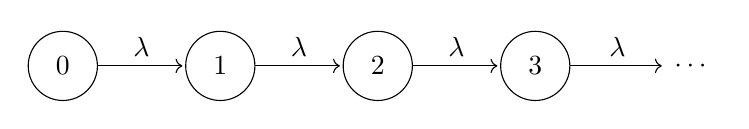
\begin{tikzpicture}[shorten >=1pt,node distance=2cm,on grid,auto] 
   \node[state] (q_0)   {$0$}; 
   \node[state] (q_1) [right=of q_0] {$1$}; 
   \node[state] (q_2) [right=of q_1] {$2$}; 
   \node[state] (q_3) [right=of q_2] {$3$};
   \node[draw=none] (q_dot) [right=of q_3] {$\cdots$};
    \path[->] 
    (q_0) edge [] node {$\lambda$} (q_1)
    (q_1) edge [] node {$\lambda$} (q_2)
    (q_2) edge [] node {$\lambda$} (q_3)
    (q_3) edge [] node {$\lambda$} (q_dot);
\end{tikzpicture}
\end{center}

As another example, consider an M/M/1 Queue. This consists of a single server whose service requirements are i.i.d Exp($\mu$) and where jobs arrive according to Poi($\lambda$). Let $X(t)$ denote the number of jobs in the system at time $t$, including the job in service. It is easy to see that $X(t)$ is a CTMC. The `timer' for arrivals or increments in $X(t)$ has a rate parameter $\lambda$ whereas the `timer' for departures or decrements in $X(t)$ has a rate parameter $\mu$. The transition rate diagram for the M/M/1 Queue is as follows

\begin{center}
    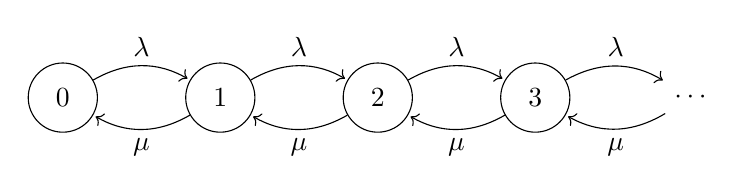
\begin{tikzpicture}[shorten >=1pt,node distance=2cm,on grid,auto] 
   \node[state] (q_0)   {$0$}; 
   \node[state] (q_1) [right=of q_0] {$1$}; 
   \node[state] (q_2) [right=of q_1] {$2$}; 
   \node[state] (q_3) [right=of q_2] {$3$};
   \node[draw=none] (q_dot) [right=of q_3] {$\cdots$};
    \path[->] 
    (q_0) edge [bend left] node {$\lambda$} (q_1)
    (q_1) edge [bend left] node {$\lambda$} (q_2)
    (q_2) edge [bend left] node {$\lambda$} (q_3)
    (q_3) edge [bend left] node {$\lambda$} (q_dot)
    (q_1) edge [bend left] node {$\mu$} (q_0)
    (q_2) edge [bend left] node {$\mu$} (q_1)
    (q_3) edge [bend left] node {$\mu$} (q_2)
    (q_dot) edge [bend left] node {$\mu$} (q_3);
\end{tikzpicture}
\end{center}

Also, the transition probability diagram for the embedded Markov chain is as follows

\begin{center}
    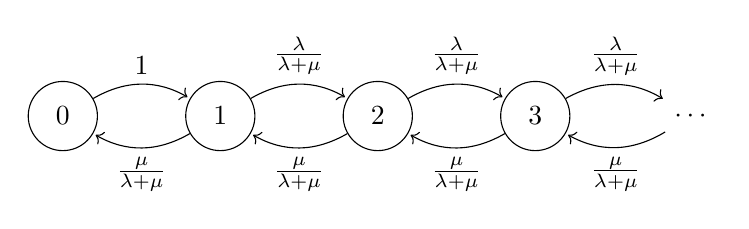
\begin{tikzpicture}[shorten >=1pt,node distance=2cm,on grid,auto] 
   \node[state] (q_0)   {$0$}; 
   \node[state] (q_1) [right=of q_0] {$1$}; 
   \node[state] (q_2) [right=of q_1] {$2$}; 
   \node[state] (q_3) [right=of q_2] {$3$};
   \node[draw=none] (q_dot) [right=of q_3] {$\cdots$};
    \path[->] 
    (q_0) edge [bend left] node {$1$} (q_1)
    (q_1) edge [bend left] node {$\frac{\lambda}{\lambda + \mu}$} (q_2)
    (q_2) edge [bend left] node {$\frac{\lambda}{\lambda + \mu}$} (q_3)
    (q_3) edge [bend left] node {$\frac{\lambda}{\lambda + \mu}$} (q_dot)
    (q_1) edge [bend left] node {$\frac{\mu}{\lambda + \mu}$} (q_0)
    (q_2) edge [bend left] node {$\frac{\mu}{\lambda + \mu}$} (q_1)
    (q_3) edge [bend left] node {$\frac{\mu}{\lambda + \mu}$} (q_2)
    (q_dot) edge [bend left] node {$\frac{\mu}{\lambda + \mu}$} (q_3);
\end{tikzpicture}
\end{center}

Now, we look at \emph{stationarity} for a CTMC. Recall that for DTMCs we found the notion of stationarity being a balance of rates quite useful. We apply the same concept here. Let $\pi$ be a ``stationary'' distribution of the CTMC. Then, for any state $i$, a simple rate balance equation gives us
\[
    \underbrace{ \pi_i \cdot \sum_{j} q_{ij} }_{\text{outgoing rates}} = \underbrace{\sum_k \pi_k \cdot q_{ki}}_{\text{incoming rates}} \iff \sum_k \pi_k \cdot q_{ki} - \pi_i \cdot \nu_i = 0
\]
Now, we define $Q \vcentcolon= [q_{ij}]$ where
\[
    q_{ij} = 
    \begin{cases}
        \nu_i \cdot p_{ij} & i \neq j \\
        -\nu_i & i=j
    \end{cases}
\]
This matrix $Q$ is called the \emph{intensity matrix}. The stationarity equations can be rewritten as
\[
    \pi \cdot Q = 0
\]
This system of equations is analogous to $\pi = \pi \cdot P$ for a DTMC. Note however that the solution to $\pi \cdot Q = 0$ is not in general the same as the solution to $\pi = \pi \cdot P$ where $P$ is the TPM of the EMC. In fact, these two are equal precisely when each state has the same rate. That is, $\nu_i = \nu$ for all $i$. 

\medskip

Notice also that $Q$ is a zero row-sum matrix. For the M/M/1 Queue, we have the following intensity matrix
\[
    Q = 
    \begin{pmatrix}
        -\lambda & \lambda & 0 & 0 & 0 & \cdots \\
        \mu & -(\lambda + \mu) & \lambda & 0 & 0 & \cdots \\
        0 & \mu & -(\lambda + \mu) & \lambda & 0 & \cdots \\
        0 & 0 & \mu & -(\lambda + \mu) & \lambda  & \cdots \\
        \vdots & \vdots & \vdots & \vdots & \vdots & \ddots
    \end{pmatrix}
\]
This matrix has $\lambda$ all along its superdiagonal, $\mu$ all along its subdiagonal and $-(\lambda + \mu)$ all along its diagonal (barring state $0$).

\subsection{Long Run Behaviour}

We again work with irreducible chains. A CTMC is said to be irreducible if the underlying EMC is irreducible. For irreducible DTMCs, we know that the existence of a stationary distribution is equivalent to meaningful long-run behaviour. However, the same is not true for CTMCs. Consider the following rate diagram:

\begin{center}
    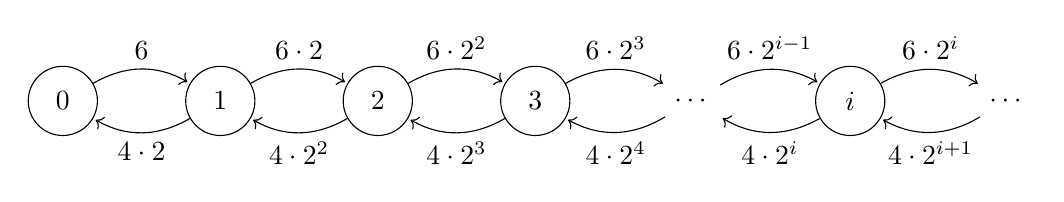
\begin{tikzpicture}[shorten >=1pt,node distance=2cm,on grid,auto] 
   \node[state] (q_0)   {$0$}; 
   \node[state] (q_1) [right=of q_0] {$1$}; 
   \node[state] (q_2) [right=of q_1] {$2$}; 
   \node[state] (q_3) [right=of q_2] {$3$};
   \node[draw=none] (q_dot1) [right=of q_3] {$\cdots$};
   \node[state] (q_i) [right=of q_dot1] {$i$};
   \node[draw=none] (q_dot2) [right=of q_i] {$\cdots$};
    \path[->] 
    (q_0) edge [bend left] node {$6$} (q_1)
    (q_1) edge [bend left] node {$6 \cdot 2$} (q_2)
    (q_2) edge [bend left] node {$6 \cdot 2^2$} (q_3)
    (q_3) edge [bend left] node {$6 \cdot 2^3$} (q_dot1)
    (q_dot1) edge [bend left] node {$6 \cdot 2^{i-1}$} (q_i)
    (q_i) edge [bend left] node {$6 \cdot 2^i$} (q_dot2)
    (q_1) edge [bend left] node {$4 \cdot 2$} (q_0)
    (q_2) edge [bend left] node {$4 \cdot 2^2$} (q_1)
    (q_3) edge [bend left] node {$4 \cdot 2^3$} (q_2)
    (q_dot1) edge [bend left] node {$4 \cdot 2^4$} (q_3)
    (q_i) edge [bend left] node {$4 \cdot 2^i$} (q_dot1)
    (q_dot2) edge [bend left] node {$4 \cdot 2^{i+1}$} (q_i);
\end{tikzpicture}
\end{center}

Using methods similar to DTMCs, we can show that the stationary distribution, satisfying $\pi \cdot Q = 0$ is given by
\[
    \pi_i = (1-\alpha) \cdot \alpha^i
\]
where $\alpha = \frac{3}{4}$. However, it is also easy to see that the underlying EMC is \emph{transient}. Note that $\nu_i = 10 \cdot 2^i$, which grows exponentially. This leads to an unbounded number of transitions in a bounded interval of time, and hence no meaningful long run behaviour. It turns out that to avoid such pathologies, it suffices to assume the recurrence of the underlying EMC. We summarise the long-run behaviour of CTMCs through the following theorem

\newpage

\begin{thm}
    Consider an irreducible CTMC with a recurrent EMC. Such a CTMC lies in either of two categories. 
    \begin{enumerate}
        \item There exists a distribution $\pi$, satisfying $\pi \cdot Q = 0$. In this case, $\pi$ is unique and positive. Additionally, $\forall \, i,j \in S$, we have
        \[
            p_{ij}(t) \xrightarrow[]{t \, \uparrow \, \infty} \pi_j
        \]
        \[
            \frac{1}{t} \int_0^t \, \mathbbm{1}_{\left\{ X(s) = i \right\}} \, ds \xrightarrow[a.s]{t \, \uparrow \, \infty} \pi_i
        \]
        In this case, $\pi$ is called the stationary, limiting and time-averaged distribution and the CTMC is said to be positive recurrent.
        
        \item There does not exist any distribution satisfying $\pi \cdot Q = 0$. In this case, $\forall \, i,j \in S$, we have
        \[
            p_{ij}(t) \xrightarrow[]{t \, \uparrow \, \infty} 0
        \]
        \[
            \frac{1}{t} \int_0^t \, \mathbbm{1}_{\left\{X(s) = i \right\}} \, ds \xrightarrow[a.s]{t \, \uparrow \, \infty} 0
        \]
        In this case, there is no meaningful long-run behaviour and the CTMC is said to be null recurrent.
    \end{enumerate}
\end{thm}

Additionally, we would like to briefly examine the \emph{transient behaviour} of a CTMC. Namely, the evolution of $p_{ij}(t)$ with time. We will assume positive recurrence. We define the matrix $P(t) \vcentcolon= [p_{ij}(t)]$. $P(t)$ can be thought as analogous to $P^{(n)}$ in the discrete-time case. Let $\mu(t)$ capture the law of the CTMC at time $t$. By the Markov property, we have
\[
    \mu(t) = \mu(0) \cdot P(t)
\]
We claim that
\[
    \frac{dP(t)}{dt} = Q \cdot P(t)
\]
The proof is left as an exercise and can be done quite easily using a $\delta$-interpretation. This then gives us a rather compact expression for $P(t)$. We have
\[
    P(t) = e^{Qt}
\]  
where the right hand side is a \emph{matrix exponential}.

\newpage

\subsection{Time Reversibility}

\begin{thm}
    Given an irreducible CTMC with recurrent EMC, if there exists a distribution $\pi$ over $S$ such that
    \[
        \pi_i \cdot q_{ij} = \pi_j \cdot q_{ji} \quad \forall \, i \in S
    \]
    then $\pi$ is the stationary distribution of the CTMC and the CTMC is positive recurrent. We call such a CTMC a \emph{time-reversible} CTMC.
\end{thm}
\begin{proof}
    We leave the proof as an exercise, since it follows along similar lines as time-reversible DTMCs.
\end{proof}

Note that the rate of $i \to j$ transitions in a CTMC is given by $\pi_i \cdot q_{ij}$. Similar to the DTMC, the stationary equation of a CTMC can be thought of as a rate balance equation. We now characterise the reverse process.

\begin{lem}
    Consider a positive recurrent CTMC. The reverse process of the CTMC is also a CTMC with 
    \[
        q^{\ast}_{ij} = \frac{\pi_j \cdot q_{ji}}{\pi_i}
    \]
\end{lem}
\begin{proof}
    Left as an exercise. Note that $\pi^{\ast} = \pi$.
\end{proof}

\begin{lem}
    For a time-reversible CTMC,
    \[
        q^{\ast}_{ij} = q_{ij}.
    \]
    That is, the reverse process is statistically identical to the forward process and has the same $Q$ matrix. (This is why these CTMCs are called time-reversible)
\end{lem}

\newpage

\section{Queueing Systems}

\subsection{Introduction}

We will use the \emph{Kendall notation} to specify queueing models. Queueing models will be denoted as $A/S/C$, where $A$ represents the interarrival time distribution, $S$ represents the service time or job size distribution and $C$ represents the number of servers. We will assume interarrival times and job sizes to be i.i.d. Occasionally, we may use an additional parameter to denote the maximum capacity of the system, as will be explained later. In these cases, queuing models will be denoted as $A/S/C/K$ where $K$ is the maximum capacity.

The distributions $A/S$ can be one of the following, for example:
\begin{enumerate}
    \item $M$ : Markovian/Memoryless
    \item $D$ : Deterministic
    \item $G$ : General
    \item Ph : Phase-type
    \item $E_k$: $k$-Erlang
\end{enumerate}

\begin{comment}


\begin{center}

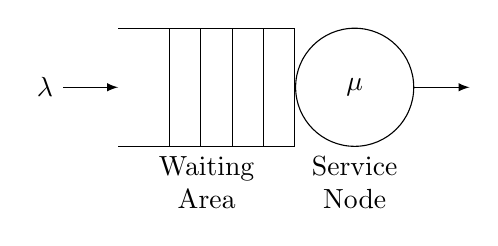
\begin{tikzpicture}[start chain=going right,>=latex,node distance=0pt]
% the rectangular shape with vertical lines
\node[rectangle split, rectangle split parts=6,
draw, rectangle split horizontal,text height=1cm,text depth=0.5cm,on chain,inner ysep=0pt] (wa) {};
\fill[white] ([xshift=-\pgflinewidth,yshift=-\pgflinewidth]wa.north west) rectangle ([xshift=-15pt,yshift=\pgflinewidth]wa.south);

% the circle
\node[draw,circle,on chain,minimum size=1.5cm] (se) {$\mu$};

% the arrows and labels
\draw[->] (se.east) -- +(20pt,0);
\draw[<-] (wa.west) -- +(-20pt,0) node[left] {$\lambda$};
\node[align=center,below] at (wa.south) {Waiting \\ Area};
\node[align=center,below] at (se.south) {Service \\ Node};
\end{tikzpicture}
\end{center}

\end{comment}

We have the two categories of performance metrics - $(i)$ \emph{System-level metrics} and $(ii)$ \emph{Job-level metrics}. Some commonly used system-level metrics are the number of jobs in queue $(N_Q)$, the number of jobs in service $(N_S)$ and the total number of jobs $(N = N_Q + N_S)$. Some commonly used job-level metrics include the waiting time or time spent in queue $(T_Q)$, the service time $(T_S)$ and the total time in system $(T = T_Q + T_S)$. The time in system, $T$, is sometimes also called the \emph{sojourn time} or \emph{response time}.

\subsection{The M/M/1 Queue}

We now consider our first queue, the $M/M/1$ queue. We have Poisson arrivals with rate $\lambda$. We have i.i.d job sizes, distributed exponentially with parameter $\mu$. We only have a single server. For now we assume FCFS (first-come-first-served) scheduling. Let $N(t)$ denote the number of jobs in the system at time $t$. It is clear that $N(t)$ is a CTMC over $\mathbb{Z}_+$. The rate diagram for this system is shown below. 

\begin{center}
    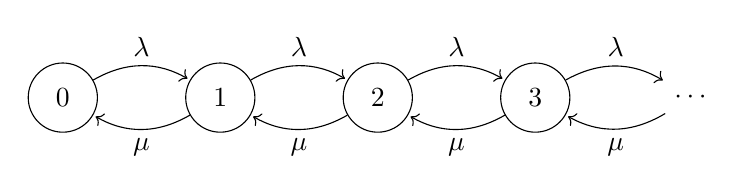
\begin{tikzpicture}[shorten >=1pt,node distance=2cm,on grid,auto] 
   \node[state] (q_0)   {$0$}; 
   \node[state] (q_1) [right=of q_0] {$1$}; 
   \node[state] (q_2) [right=of q_1] {$2$}; 
   \node[state] (q_3) [right=of q_2] {$3$};
   \node[draw=none] (q_dot) [right=of q_3] {$\cdots$};
    \path[->] 
    (q_0) edge [bend left] node {$\lambda$} (q_1)
    (q_1) edge [bend left] node {$\lambda$} (q_2)
    (q_2) edge [bend left] node {$\lambda$} (q_3)
    (q_3) edge [bend left] node {$\lambda$} (q_dot)
    (q_1) edge [bend left] node {$\mu$} (q_0)
    (q_2) edge [bend left] node {$\mu$} (q_1)
    (q_3) edge [bend left] node {$\mu$} (q_2)
    (q_dot) edge [bend left] node {$\mu$} (q_3);
\end{tikzpicture}
\end{center}

For stability of the system, we require positive recurrence of the CTMC. Hence, the system is stable if and only if $\lambda < \mu$. We leave the calculation of the stationary distribution as an exercise to the reader. Verify that the stationary distribution is given by
\[
    \pi_n = (1-\rho) \cdot \rho^n \text{ for all } n 
\]
where $\rho = \frac{\lambda}{\mu}$ is called the \emph{utilisation} of the system. Note that the long run fraction of time that the server is busy is given by $(1-\pi_0) = \rho$, which is precisely why $\rho$ is called the utilisation.

Let $N$ be the steady-state number of jobs in the system. The p.m.f of $N$ is precisely the stationary distribution $\pi$ of the system. Now,
\[
    \E[N] = \sum_{k=0}^{\infty} k(1-\rho)\rho^k = \frac{\rho}{1-\rho}
\]
This is the steady-state average number of jobs in the system. We see that as $\rho \uparrow 1$, $\E[N] \uparrow \infty$. That is, as the system approaches the limit of stability, the steady-state average number of jobs in the system grows without bound. We leave it as an exercise to the user to calculate $\E[T]$ for the $M/M/1$ queue (Hint: Wald's Lemma).

\subsection{Little's Law}

We now state and prove a fundamental result in Queueing Theory, namely, Little's law. Informally, this states that for any system, the time-averaged number of ``jobs'' in the system equals the product of the time-averaged arrival rate and the time-averaged time spent in the system. This idea is formalised below.

\begin{thm}[Little's Law]
    Let $N(t)$ denote the number of `items' or `jobs' in a system at time $t$. Let $A(t)$ denote the number of arrivals to the system up to time $t$ and let $D(t)$ denote the number of departures from the system up to time $t$. Let $W_i$ be the time spent in the system by the $i^{\text{th}}$ arrival. Suppose, on a sample path, we have
    \[
        \lim_{t \to \infty} \frac{A(t)}{t} = \lim_{t \to \infty} \frac{D(t)}{t} = \lambda
    \]
    and suppose 
    \[
        \overline{W} = \lim_{n \to \infty} \frac{1}{n} \sum_{i=1}^n W_i
    \]
    Then,
    \[
        \overline{N} \vcentcolon= \lim_{t \to \infty} \frac{1}{t} \int_0^t N(s) \, ds = \lambda \cdot \overline{W}
    \]  
\end{thm}
\begin{proof}
    This is essentially a pictorial proof. Corresponding to the time spent in the system by each arrival, draw a rectangle of height $1$ over the timeline, vertically stacked. Under this construction, $N(t)$ will be the number of rectangles encountered vertically at time $t$. Moreover, the integral
    \[
        \int_0^t N(s) \, ds 
    \]
    is the area occupied by the rectangles to the left of $t$ (including any `incomplete' rectangles). With this, we have the following bound.
    \[
        \sum_{i=1}^{D(t)} W_i \leq \int_0^t N(s) \, ds \leq \sum_{i=1}^{A(t)} W_i
    \]
    This follows since the LHS does not include the `incomplete' rectangles whereas the RHS includes the entire area occupied by the `incomplete' rectangles. The integral is then sandwiched between these two quantities. We then have    
    \[
        \frac{1}{t} \sum_{i=1}^{D(t)} W_i \leq \frac{1}{t} \int_0^t N(s) \, ds \leq \frac{1}{t} \sum_{i=1}^{A(t)} W_i
    \]
    \[
        \therefore \, \frac{D(t)}{t} \cdot \frac{1}{D(t)}\sum_{i=1}^{D(t)} W_i \leq \frac{1}{t} \int_0^t N(s) \, ds \leq \frac{A(t)}{t} \cdot \frac{1}{A(t)} \sum_{i=1}^{A(t)} W_i
    \]
    Taking limit $t \uparrow \infty$ on either side, the first term becomes $\lambda$ and the second term becomes $\overline{W}$. Hence, 
    \[
        \lim_{t \to \infty} \frac{1}{t} \int_0^t N(s) \, ds = \lambda \cdot \overline{W} \qedhere
    \]
\end{proof}

Notice that this is purely a sample-path based result and does not need a probability space. In ergodic systems, these time averages also match ensemble averages. That is,
\[
    \overline{N} = \E[N] \text{ almost surely and  } \overline{W} = \E[W] \text{ almost surely.}
\]

We now apply Little's Law to the $M/M/1$ system. We consider our system to be the waiting area along with the server. Clearly, the arrival rate into the system is $\lambda$. We calculated $\E[N]$ previously. By Little's Law, we get
\[
    \E[T] = \frac{1}{\lambda} \E[N] \implies \boxed{\E[T] = \frac{1}{\lambda} \cdot \frac{\rho}{1-\rho} = \frac{1}{\mu - \lambda}}
\]

Alternatively, consider that our system consists of only the server. Again, the arrival rate into the system is $\lambda$ while the average time spent in the system is simply the expected service time, or $\frac{1}{\mu}$. By Little's Law, we have
\[
    \E[N] = \lambda \cdot \frac{1}{\mu} = \rho
\]
However, $\E[N]$ is simply the time-averaged number of jobs that are there in the system or server. This is same as the long-run fraction of time the server is busy or the time-averaged occupancy of the system. We had computed this number earlier using the stationary distribution. However, Little's Law allows us to obtain the same result in a much simpler way.

Consider that we scale the service and arrival rates proportionately. That is, instead of $\lambda, \mu$ we have $k\lambda, k\mu$ for some scaling factor $k$. In this case, $\rho$, which is the ratio of the two, remains unchanged. Hence, the steady-state expected number of jobs in the system remains unchanged. However, the expected time spent in the system decreases by a factor of $k$. One may interpret this `scaling' of arrival and service rates as simply fast-forwarding the original system a factor of $k$. As expected, this would have no bearing on the expected number of jobs in the system but would modify the expected response time by a factor of exactly $k$.

\subsection{Poisson Arrivals See Time Averages}

We now state a crucial property of Poisson arrivals. Let $p_n$ denote the long-run fraction of time there are $n$ jobs in the system and let $a_n$ be the long-run fraction of arrivals that see $n$ jobs in the system on arrival. We claim that if the arrivals occur according to a Poisson process, then $p_n = a_n$. This is formalised by the theorem below called the Arrival Theorem or the PASTA property (Poisson Arrivals See Time Averages). 

\begin{thm}[PASTA]
    Suppose $\left\{ X(t) \right\}_{t \geq 0}$ is a stochastic process taking values in $S$. Suppose that the sample paths of $X$ are right continuous with left limits. Suppose $\left\{N(t)\right\}_{t \geq 0}$ is a Poisson process. \emph{Lack of Anticipation Assumption (LAA):} For any $t \geq 0$, arrivals post $t$ are independent of the state of the system prior to $t$. That is,
    \[
        N(t+u) - N(t) \indep \left\{ X(s) \mid 0 \leq s \leq t \right\} \text{ for all } u \geq 0
    \]
    Let $B \subseteq S$ be measurable. We define
    \[
        \mathbbm{1}_{B}(t) \vcentcolon= \begin{cases}
            1 & \text{if } X(t) \in B \\
            0 & \text{otherwise}
        \end{cases}
        \quad \text{and} \quad
        \mathbbm{1}_B^{(n)} \vcentcolon= \begin{cases}
            1 & \text{if $n^{\text{th}}$ arrival sees } X(t) \in B \\
            0 & \text{otherwise}
        \end{cases}
    \]
    Assuming LAA, the following is true
    \begin{align*}
        \lim_{t \to \infty} \frac{1}{t} \int_0^t \mathbbm{1}_B(s) \, ds &= p_B \text{ almost surely} \\
        &\Big\Updownarrow \\
        \lim_{n \to \infty} \frac{1}{n} \sum_{k=1}^n \mathbbm{1}_B^k &= p_B \text{ almost surely}
    \end{align*}
\end{thm}

Informally, PASTA says that the system average and the customer average match with probability $1$, so long as one of them exists. To see the power of this theorem, consider the following question. For the M/M/1 queue, what is the long run fraction of jobs that do not have to wait? This is the long run fraction of arrivals that see the system to be in empty. By PASTA, this is precisely $\pi_0$. Moreover, PASTA is also crucial in simulations. To estimate the time-averaged distribution of a system, we only need to view the system at the arrival instants.

\subsection{Erlang Models}

In $1917$, A.K. Erlang published a single paper that contained three classic formulae, namely Erlang models A,B, and C, corresponding to three queueing systems. These formulae are in use even today in telephony and cellular services. In fact, it is not an overstatement to say that Erlang's work marks the birth of queueing theory. We now study two of these three models.
\
\subsubsection{The Erlang-B Model}

The Erlang-B Model, in the Kendall notation, is the M/M/$k/k$ queue. Jobs arrive as per a Poisson process of rate $\lambda$. We have $k$ servers, each having i.i.d Exp($\mu$) service times. Since the capacity of the system is $k$ as well, when a job arrives, it begins service at a free server if one is available. Else, the job is dropped. Since this model is frequently used to model telephony, we refer to jobs as `calls'. Hence, when the system is operating at full capacity and a new call arrives, the call is dropped, as has so often happened to all of us. Our objective is to characterise the fraction of calls that are dropped. 

The number of busy servers in the system evolves as a CTMC, as per the following rate diagram.

\begin{center}
    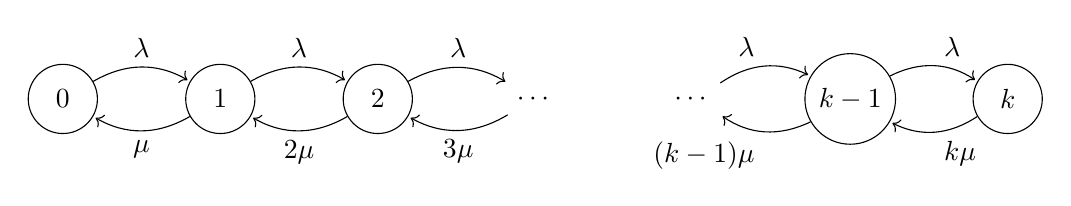
\begin{tikzpicture}[shorten >=1pt,node distance=2cm,on grid,auto] 
   \node[state] (q_0)   {$0$}; 
   \node[state] (q_1) [right=of q_0] {$1$}; 
   \node[state] (q_2) [right=of q_1] {$2$}; 
   \node[draw=none] (q_dot) [right=of q_2] {$\cdots$};
   \node[draw=none] (q_dot2) [right=of q_dot] {$\cdots$};
   \node[state] (q_k1) [right=of q_dot2] {$k-1$};
   \node[state] (q_k) [right=of q_k1] {$k$};
    \path[->] 
    (q_0) edge [bend left] node {$\lambda$} (q_1)
    (q_1) edge [bend left] node {$\lambda$} (q_2)
    (q_2) edge [bend left] node {$\lambda$} (q_dot)
    (q_dot2) edge [bend left] node {$\lambda$} (q_k1)
    (q_k1) edge [bend left] node {$\lambda$} (q_k)
    (q_1) edge [bend left] node {$\mu$} (q_0)
    (q_2) edge [bend left] node {$2\mu$} (q_1)
    (q_dot) edge [bend left] node {$3\mu$} (q_2)
    (q_k1) edge [bend left] node {$(k-1)\mu$} (q_dot2)
    (q_k) edge [bend left] node {$k\mu$} (q_k1);
    
\end{tikzpicture}
\end{center}

Using the time-reversibility equation, we obtain for the stationary distribution
\[
    \pi_i \cdot \lambda = \pi_{i+1} \cdot (i+1)\mu \quad (0 \leq i < k)
\]
Thus, 
\[
    \pi_i = \pi_0 \cdot \frac{a^i}{i!}
\]
where $a = \frac{\lambda}{\mu}$. On normalising, we get
\[
    \pi_0 = \left( \sum_{i=0}^k \frac{a^i}{i!} \right)^{-1}
\]

By PASTA, the long run fraction of calls that are dropped is simply $\pi_k$. We denote this number as $\mathcal{B}(a,k)$, the \emph{blocking probability}. The blocking probability is given by the Erlang-B formula, as follows
\[
    \boxed{\mathcal{B}(a,k) = \ddfrac{a^k/k!}{\sum_{i=0}^k \frac{a^i}{i!}}}
\]

Note that the M/M/k/k system is always stable and increasing $a$ simply increases $\mathcal{B}(a,k)$. It is convenient to represent $\mathcal{B}(a,k)$ in terms of a Poisson random variable, as follows. Let $X \sim \text{Poi}(a)$. Then, 
\[
    \mathcal{B}(a,k) = \frac{\P(X = k)}{\P(X \leq k)}
\]

Note that in practice, the assumption of Poisson arrivals is reasonable but assuming an exponential call duration is not. However, what makes the Erlang-B formula so powerful is that it holds for any generic call duration distribution with mean $\frac{1}{\mu}$.

\subsubsection{The Erlang-C Model}

The Erlang-C Model, in the Kendall notation, is the M/M/$k$ queue. Jobs arrive as per a Poisson process of rate $\lambda$. We have $k$ servers, each having i.i.d Exp($\mu$) service times. We have a single, infinite capacity queue. Jobs are scheduled as per the FCFS policy. The number of jobs in the system evolves as a CTMC, with the following rate diagram.


\begin{center}
    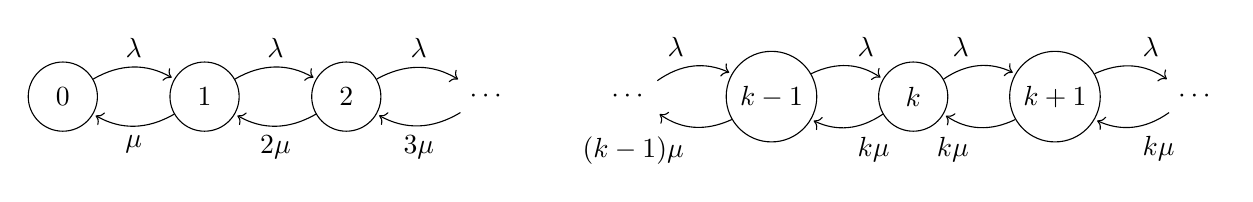
\begin{tikzpicture}[shorten >=1pt,node distance=1.8cm,on grid,auto] 
   \node[state] (q_0)   {$0$}; 
   \node[state] (q_1) [right=of q_0] {$1$}; 
   \node[state] (q_2) [right=of q_1] {$2$}; 
   \node[draw=none] (q_dot) [right=of q_2] {$\cdots$};
   \node[draw=none] (q_dot2) [right=of q_dot] {$\cdots$};
   \node[state] (q_k1) [right=of q_dot2] {$k-1$};
   \node[state] (q_k) [right=of q_k1] {$k$};
   \node[state] (q_k2) [right=of q_k] {$k+1$};
   \node[draw=none] (q_dot3) [right=of q_k2] {$\cdots$};
    \path[->] 
    (q_0) edge [bend left] node {$\lambda$} (q_1)
    (q_1) edge [bend left] node {$\lambda$} (q_2)
    (q_2) edge [bend left] node {$\lambda$} (q_dot)
    (q_dot2) edge [bend left] node {$\lambda$} (q_k1)
    (q_k1) edge [bend left] node {$\lambda$} (q_k)
    (q_1) edge [bend left] node {$\mu$} (q_0)
    (q_2) edge [bend left] node {$2\mu$} (q_1)
    (q_dot) edge [bend left] node {$3\mu$} (q_2)
    (q_k1) edge [bend left] node {$(k-1)\mu$} (q_dot2)
    (q_k) edge [bend left] node {$k\mu$} (q_k1)
    (q_k) edge [bend left] node {$\lambda$} (q_k2)
    (q_k2) edge [bend left] node {$\lambda$} (q_dot3)
    (q_dot3) edge [bend left] node {$k\mu$} (q_k2)
    (q_k2) edge [bend left] node {$k\mu$} (q_k);
    
\end{tikzpicture}
\end{center}

We define 
\[
    a \vcentcolon= \frac{\lambda}{\mu} \text{ and } \rho \vcentcolon= \frac{\lambda}{k\mu}
\]
By Little's Law, $\rho$ is the utilisation, the fraction of time each server is busy. For stability of the system, we need
\[
    \rho < 1 \iff a < k \iff \lambda < k\mu.
\]By time reversibility, we get
\[
    \pi_i = \begin{cases}
        \frac{a^i}{i!} \cdot \pi_0 & i < k \\
        \frac{a^i}{k! k^{i-k}} \cdot \pi_0 & i \geq k
    \end{cases}
\]
On normalising, we have
\[
    \pi_0^{-1} = \sum_{i=0}^k \frac{a^i}{i!} + \sum_{i=k}^{\infty} \frac{a^i}{k!k^{i-k}} = \sum_{i=0}^k \frac{a^i}{i!} + \frac{a^k}{k!} \sum_{i=k}^{\infty} \left( \frac{a}{k} \right)^{i-k}
\]
Thus,
\[
    \pi_0 = \left( \sum_{i=0}^k \frac{a^i}{i!} + \frac{a^k}{k!(1-\rho)} \right)^{-1}
\]

By PASTA, the long run fraction of jobs that have to wait is simply the fraction of time the system spends in states greater than or equal to $k$. We denote this number as $\mathcal{C}(a,k)$. We have
\[
    \mathcal{C}(a,k) = \sum_{i\geq k} \pi_i
\]
On simplifying, we get the Erlang-C Formula.
\[
    \boxed{\mathcal{C}(a,k) = \ddfrac{\frac{a^k}{k!(1-\rho)}}{\sum_{i=0}^k \frac{a^i}{i!} + \frac{a^k}{k!(1-\rho)}}}
\]

For $a < k$, we may rewrite the Erlang-C formula in terms of the Erlang-B formula, as follows.
\[
    \mathcal{C}(a,k) = \frac{\mathcal{B}(a,k)}{1-\rho + \rho\cdot\mathcal{B}(a,k)}
\]
Note that although $\mathcal{B}(a,k)$ is well-defined for $a \geq k$, the above relation is valid only for $a < k$. We leave the proof of the above expression as an exercise. The reader may find it helpful to appeal to the Poisson-random-variable version of the Erlang-B formula.

Let us now compute the steady-state metrics of the system. Conditioned on $N \geq k$, we have
\begin{align*}
    \P(N_Q = i \mid N \geq k) &= \P(N = k+i \mid N \geq k) \\
    &= \frac{\P(N=k+i)}{\P(N\geq k)} \\
    &= \ddfrac{\frac{a^{k+i}}{k!k^i}}{\frac{a^k}{k!(1-\rho)}} \\
    &= \rho^i (1-\rho)
\end{align*}
This is exactly the same distribution as the M/M/1 queue, which should not be surprising. We then have
\[
    \E[N_Q \mid N \geq k] = \frac{\rho}{1-\rho} \implies \E[N_Q] = \P(N \geq k) \cdot \E[N_Q \mid N \geq k]
\]
This gives us
\[
    \E[N_Q] = \mathcal{C}(a,k) \cdot \frac{\rho}{1-\rho}
\]
    
Applying Little's Law, we get
\[
    \E[T_Q] = \frac{\mathcal{C}(a,k)}{k\mu - \lambda}
\]
Now, 
\[
    \E[T] = \E[T_Q] + \E[T_S] = \frac{\mathcal{C}(a,k)}{k\mu-\lambda} + \frac{1}{\mu}
\]
Again, applying Little's Law, we get
\[
    \E[N] = \E[N_Q] + a
\]
Thus, the expected number of jobs in service is $a$. In fact, this could have been easily proved using Little's Law on all of the $k$ servers.

\subsection{The M/G/1 Queue}

We will now study the M/G/1 queue. Jobs arrive as per a Poisson process of rate $\lambda$. Job sizes are i.i.d, independent of the arrival process, and have a generic distribution. We define 
\[
    \rho \vcentcolon= \lambda \E[X].
\]
For stability, we need $\rho < 1$. Note that $\rho$ is the long term rate at which work comes into the system. This can be seen formally using the Renewal-Reward Theorem, considering renewals to be arrivals into the queue and the reward in epoch $n$ to be the size of the $n^{\text{th}}$ job. By Little's Law, $\rho$ is also the long run fraction of time the server is busy. 

We wish to compute $\E[T_Q]$, the steady state expected wait time. Note that
\[
    T_Q = \sum_{i=1}^{N_Q^A} X_i + L^A
\]
where $N_Q^A$ is the number of jobs in the queue as seen by an arriving job, in steady state, and $L^A$ is the residual service time of the job in service as seen by an arriving job, in steady state. Since $N_Q^A$ is independent of $X_i$'s, we may apply Wald's Lemma to obtain
\[
    \E[T_Q] = \E[N_Q^A] \cdot \E[X] + \E[L^A]
\]
By PASTA, we have
\[
    \E[T_Q] = \E[N_Q] \cdot \E[X] + \E[L]
\]
By Little's Law, we have
\[
    \E[T_Q] = \lambda \E[T_Q] \cdot \E[X] + \E[L] \implies \E[T_Q] = \frac{\E[L]}{1-\rho}
\]
Hence, it remains to find $\E[L]$. We leave the details of this computation as an exercise to the reader. Consider renewal instants to be the instants when the system enters a ``busy period'' and considering $L(t)$ to be the reward signal. On using a sandwich-based argument, similar to the proof of Little's Law, we conclude that
\[
    \E[L] = \frac{\lambda \E[X^2]}{2}
\]
This gives us
\[
    \boxed{\E[T_Q] = \frac{\lambda \E[X^2]}{2(1-\rho)}}
\]
which is commonly referred to as the \textbf{Pollaczek-Khinchine Formula}. Notice that the mean wait time increases with job size variability. Next, we compute the steady state expected busy period of the system. We define renewal instants at instants when the server enters a busy period. If $B$ denotes the length of a busy period and $I$ denotes the length of an idle period, then the length of a renewal cycle is $B+I$. Let the reward signal be defined as
\[
    R(t) = \mathbbm{1}_{\left\{\text{server is busy at time }t\right\}}
\]
Thus, the expected reward in a single renewal cycle is $\E[B]$. By Little's Law,
\[
    \frac{1}{t} \int_0^t R(s) \, ds \xrightarrow{t \, \uparrow \, \infty}[a.s] \rho
\]
By the Renewal-Reward Theorem, 
\[
    \rho = \frac{\E[B]}{\E[B] + \E[I]} = \frac{\E[B]}{\E[B] + \frac{1}{\lambda}}
\]
This gives us
\[
    \E[B] = \frac{\E[X]}{1-\rho}
\]

\subsection{Scheduling Policies}

We take a short excursion from queueing models and talk about scheduling policies. So far, we have considered only the FCFS scheduling policies. In practice, we have a plethora of options to choose from. We classify scheduling policies as follows.

\begin{itemize}
    \item \begin{enumerate}
        \item \underline{Non-preemptive}: A non-preemptive policy does not allow a job to be interrupted once it has begun service.
        \item \underline{Preemptive}: A preemptive policy allows service to be interrupted and resumed later.
    \end{enumerate}
    
    \item \begin{enumerate}
        \item \underline{Blind}: A blind policy does not make use of job size information in scheduling.
        \item \underline{Size-based}: A size-based policy uses job size information to schedule jobs.
    \end{enumerate}
\end{itemize}

We will not dive into the details of scheduling policies, but we will state two important results, before moving on. The reader is encouraged to study these policies in detail.

\begin{thm}
    In the M/G/1 queue, all non-preemptive, blind policies have the same $\E[T_Q]$ as the FCFS scheduling policy. However, they do not have the same distribution for $T_Q$. Among non-preemptive, blind policies, the FCFS policy minimises $\Var{T_Q}$ for a given $\E[T_Q]$. 
\end{thm}

It turns out that the `optimal' policy is a preemptive, size-based policy known as the SRPT policy (Shortest Remaining Processing Time). As the name suggests, this policy provides service to that job which has the shortest remaining processing time. For the SRPT policy, we have the following crucial result.

\begin{thm}
    On any arrival sequence,
    \[
        \E\left[ T^{SRPT} \right] \leq \E\left[ T^P \right]
    \]
    under any scheduling policy $P$.
\end{thm}
This theorem follows easily from the following Lemma, using Little's Law

\begin{lem}
    On any arrival sequence, for any policy $P$,
    \[
        N^{SRPT}(t) \leq N^P(t) \quad \forall \, t.
    \]
\end{lem}

We omit the proof here. Note that no stochastic assumptions have been made. The SRPT policy is optimal under the G/G/1 queue, as well as adversially chosen arrival sequences.

\subsection{Burke's Theorem and Queueing Networks}

Finally, we study queueing networks. Throughout the remainder, we assume that jobs are scheduled according to the FCFS policy, at each server. Perhaps the simplest queueing network problem is that of tandem queues. Consider that we have two infinite-capacity queues, $1$ and $2$. Jobs arrive into queue $1$ according to a Poisson process of rate $\lambda$. Queue $1$ has a single server whose service times are i.i.d Exp($\mu_1$). Jobs that finish service in queue $1$ move over to queue $2$, which again has a single server whose service times are i.i.d Exp($\mu_2$). We wish to analyse the steady state job distribution  of this system. The obvious solution is to model the system as a $2$-dimensional CTMC where the state of the system is the $2$-tuple $(n_1, n_2)$ corresponding to the number of jobs in each queue. The problem with this solution is that it is tedious, and it does not generalise to larger networks. We now explore a much simpler solution, based on characterising the departure process of the first queue. This exploits the concept of time-reversibility. Notice that the M/M/1 CTMC is indeed time-reversible. This gives us the following result.

\begin{thm}[Burke's Theorem]
    For an M/M/1 queue with arrival rate $\lambda$, the following are true in steady state.
    \begin{enumerate}
        \item The departure process is Poisson with rate $\lambda$.
        \item At all $t$, $N(t)$ is independent of past departures.
    \end{enumerate}
\end{thm}

\begin{proof}
    \phantom{hi}
    \begin{enumerate}
        \item Since the CTMC is time-reversible, the reverse process is statistically identical to the forward process. Hence, the arrival process of the reverse process is Poi($\lambda$). Since this is the same as the departure process of the forward process, the firs part follows.
        
        \item Departures prior to time $t$ in the forward process are arrivals after time $t$ in the reverse process. However, $N(t)$ is independent of future arrivals in the reverse process.
    \end{enumerate}
\end{proof}

Let us get back to our tandem system. By Burke's Theorem, the departure process of queue $1$ is Poi($\lambda$) and hence queue $2$ is also an M/M/1 queue. Moreover, $N_2(t)$ is completely determined by the departures of queue $1$. Since $N_1(t)$ is independent of these departures, the two queues are completely independent M/M/1 queues. Let $N = (N_1, N_2)$ be the stationary job distribution in the system. We then have
\[
    \P\left( N_1 = n_1, N_2 = n_2 \right) = (1-\rho_1)\rho_1^{n_1} \cdot (1-\rho_2)\rho_2^{n_2}
\]
where 
\[
    \rho_1 = \frac{\lambda}{\mu_1} \text{ and } \rho_2 = \frac{\lambda}{\mu_2}
\]

In fact, these nice results hold for any acyclic network. Consider for example, the following network in shown in Figure \ref{fig:acyclic}

\begin{figure}[!h]
    \centering
    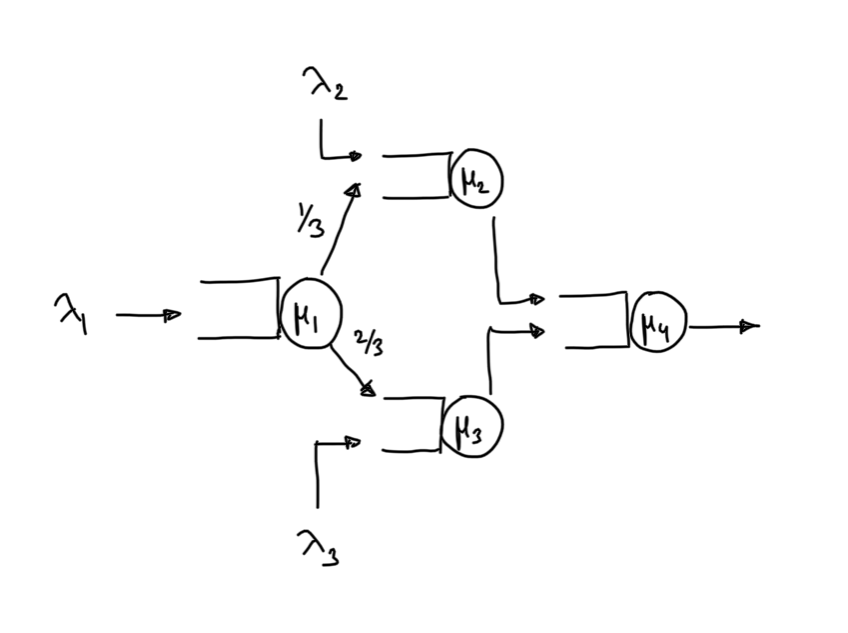
\includegraphics[width=0.6\linewidth]{AcyclicNetwork.PNG}
    \caption{An example acyclic network}
    \label{fig:acyclic}
\end{figure}

Each of the four queues is an independent M/M/1 queue. We define
\begin{align*}
    \rho_1 &= \frac{\lambda_1}{\mu_1} \\
    \rho_2 &= \frac{\lambda_2 + 1/3\lambda_1}{\mu_2} \\
    \rho_3 &= \frac{\lambda_3 + 2/3\lambda_1}{\mu_3} \\
    \rho_4 &= \frac{\lambda_1 + \lambda_2 + \lambda_3}{\mu_4}
\end{align*}
Then, the state of the system, $N = (N_1, N_2, N_3, N_4)$ has the following distribution.
\[
    \P\left( N_i = n_i , i = 1, \ldots, 4 \right) = \prod_{i=1}^4 (1-\rho_i) \cdot \rho_i^{n_i}
\]



\end{document}

